%
% File acl2015.tex
%
% Contact: car@ir.hit.edu.cn, gdzhou@suda.edu.cn
%%
%% Based on the style files for ACL-2014, which were, in turn,
%% Based on the style files for ACL-2013, which were, in turn,
%% Based on the style files for ACL-2012, which were, in turn,
%% based on the style files for ACL-2011, which were, in turn,
%% based on the style files for ACL-2010, which were, in turn,
%% based on the style files for ACL-IJCNLP-2009, which were, in turn,
%% based on the style files for EACL-2009 and IJCNLP-2008...

%% Based on the style files for EACL 2006 by
%%e.agirre@ehu.es or Sergi.Balari@uab.es
%% and that of ACL 08 by Joakim Nivre and Noah Smith

\documentclass[11pt]{article}
\usepackage{acl2015}
\usepackage{times}
\usepackage{hyperref}
\usepackage{latexsym}
\usepackage{color}
\usepackage{amsmath}
\usepackage{epsfig}
\usepackage{graphicx}
\newcommand{\figref}[1]{Figure \ref{#1}}
\newcommand{\tabref}[1]{Table \ref{#1}}
\usepackage{epstopdf}
\usepackage{booktabs}
\usepackage{diagbox}
\usepackage{array}
%\usepackage{float}
\usepackage{stfloats}
\usepackage{multicol}
\usepackage{threeparttable}
\usepackage[multiple]{footmisc}

%\usepackage[skip=2pt,font=scriptsize]{caption}
\newcolumntype{I}{!{\vrule width 1pt}}
\newlength\savedwidth
\newcommand\whline{\noalign{\global\savedwidth\arrayrulewidth
                            \global\arrayrulewidth 1pt}%
                   \hline
                   \noalign{\global\arrayrulewidth\savedwidth}}
\newlength{\Oldarrayrulewidth}
\newcommand{\Cline}[2]{%
  \noalign{\global\setlength{\Oldarrayrulewidth}{\arrayrulewidth}}%
  \noalign{\global\setlength{\arrayrulewidth}{#1}}\cline{#2}%
  \noalign{\global\setlength{\arrayrulewidth}{\Oldarrayrulewidth}}}

\newcommand{\KZ}[1]{\textcolor{blue}{Kenny: #1}}
\newcommand{\BF}[1]{\textcolor{red}{Bean: #1}}
\newcommand{\TJ}[1]{\textcolor{red}{Jia: #1}}
\newcommand{\YZ}[1]{\textcolor{red}{Yizhong: #1}}
\newcommand{\cut}[1]{}


% You can expand the titlebox if you need extra space
% to show all the authors. Please do not make the titlebox
% smaller than 5cm (the original size); we will check this
% in the camera-ready version and ask you to change it back.


\title{BeanParser: A Sequence-based Dependency Parser}

\author{Wenjing Fang \and Yizhong Wang \and Jia Tan \and Kenny Q. Zhu  \\
  Shanghai Jiao Tong University \\
  {\tt littlebeanfang@sjtu.edu.cn}, {\tt kzhu@cs.sjtu.edu.cn} \\
  }
%\date{}

\begin{document}
\maketitle
\begin{abstract}
%Existing data-driven dependency parsers mainly fall into two classes:
%graph-based and transition-based. However, both methods draw some distinctions
%from the way that we human beings perform the parsing task.
This paper demonstrates a novel dependency parsing framework that
imitates how a human parses sentences in an intuitive way.
At every step of the parse, it determines which word is the easiest to
process among all the remaining words, identifies its head word and then
folds it under the head word.
This greedy framework achieves competitive accuracy on WSJ evaluation set
and shows additional advantage on the non-projective corpus.
%\BF{multi-lingual}
 % \BF{redo experiment,not the accurate number}
Further, this work is flexible enough to be augmented with other
parsing techniques.
\end{abstract}
%\IEEEraisesectionheading{
% %\IEEEraisesectionheading{
% %\IEEEraisesectionheading{
% \input{intro}
\section{Introduction}\label{sec:intro}
 %}
% \section{Introduction}\label{sec:intro}

% \begin{enumerate}
% \item Motivation: application scenarios (with 1-2 running examples);
% \item Characteristics of the data sources and their challenges;
% \item Briefly introduce previous approaches to extract information 
% from images including setting the document zone, and their limitations.
% \item General flow of our approach (may give a diagram here)
% \end{enumerate}
% scenary

Due to ever evolving hardware and software, many medical images
such as electro-cardio graphs (ECGs), X-ray or ultrasound images  
are directly printed and stored in hard copy formats. 
% \KZ{Insert 4 example images here.}
%Examples are shown in \figref{fig:medicalImages}. 
% These images often contain a mix of graphics and text, which
% include parameter settings of the hardware, test measurements or simple
% diagnosis. 
These images often contain a mix of graphics and text, which 
include technical settings of the hardware used, test measurements or simple diagnoses.
Recently, there has been a growing demand for digitizing such 
medical information from paper media sources, especially legacy ones, or patients who want to keep track of these documents by themselves digitally. 
Apart from scanning the graphics into a digital format, extracting 
the semi-structured textual information is also an important part of
building electronic medical records for patients. 

%\begin{figure}[!htb]
%\centering
%\subfloat[ECG]{
%\label{fig:medicalimage:ecg}
%\epsfig{file=figure/17_ori.eps, width=0.4\columnwidth}
%}
%% \hfill
%\subfloat[MRI]{
%	\label{fig:medicalimage:mrt}
%	\epsfig{file=figure/MRI.eps, width=0.4\columnwidth}
%}
%\\
%\subfloat[X-RAY]{
%\label{fig:medicalimage:xray}
%\epsfig{file=figure/X-RAY.eps, width=0.4\columnwidth}
%}
%%\hfill
%\subfloat[EEG]{
%\label{fig:medicalimage:eeg}
%\epsfig{file=figure/EEG.eps, width=0.4\columnwidth}
%}
%\caption{Examples of Medical Images}
%\label{fig:medicalImages}
%\end{figure}

Optical character recognition (OCR)  \cite{mori1992historical,smith2007overview} is 
a traditional technique used to turn images of printed text into machine encoded
text. It is well researched and performs well on plain text 
documents such as novels and reports, for a variety of languages. 
%For example, Tesseract, which is one of 
%the most popular open source multilingual recognizers, logs an error 
%rate of 3.72\% for English words and 3.77\% for simplified 
%Chinese characters\cite{smith2009adapting}. 
%Google Books \cite{googlebooks} and Gutenberg \cite{gutenberg} are
%projects which have scanned a large number of paper books into text for free and open
%access. These projects made exclusive use of OCR for this conversion and 
%achieved high accuracy \cite{vincent2007google} \cite{lebert2008project}. 
% 99\% for Gutenberg project \cite{lebert2008project}. 
% \KZ{Give the accuracy of google and gutenberg if available.}


\begin{figure}[th]
\centering
\epsfig{file=figure/17_b.eps, width=0.8\columnwidth}
\caption{An ECG image with text area (red circle) of interest.}
\label{fig:ecgexample2}
\end{figure}

For a semi-structured medical image, such as 
\figref{fig:ecgexample2}, we would like to extract the attribute-value 
pairs (e.g., {\em Vent. rate = 63 bpm}) and possibly other values such as
date ({\em 18-Nov-2010}) and time ({\em 9:13:02}) since those values endow us with lots of information about the patient. 
Existing OCR software cannot extract such structured information in a straightforward 
fashion, 
but instead it produces rather convoluted results from the whole image, 
similar to those in \figref{fig:ocrre}, which was produced by Tesseract, 
a popular multi-lingual recognizers. 
% \KZ{Maybe include the x-y coordinate info in the output as well?}  

\begin{figure}[th]
\centering
\scriptsize
\begin{verbatim}
<p class="ocr_par" title="box 263 33 444 119">
   <span class="ocr_l" title="box 264 33 336 45">
       <span class="ocrx_w" title="box 264 33 299 45">Vcnt.</span> 
       <span class="ocrx_w" title="box 308 34 336 45">rule</span> 
   </span>
   <span class='ocr_l'>
       <span class="ocrx_w" title="box 264 51 283 64">PR</span> 
       <span class="ocrx_w" title="box 291 51 346 64">Interval</span> 
       <span class="ocrx_w" title="box 389 52 411 64">140</span> 
       <span class="ocrx_w" title="box 420 55 439 64">ms</span> 
   </span>
   ...
   </span>
</p>
<p class="ocr_p" dir="ltr">
   <span class="ocr_l">
       <span class="ocrx_w" title="box 396 33 411 45">53</span> 
       <span class="ocrx_w" title="box 420 33 449 48">bpm</span> 
   </span>
</p>
\end{verbatim}
\caption{Snippet OCR results in XML, input to our framework.}
\label{fig:ocrre}
\end{figure}


%\input{xmlre1}

%However, OCR alone does not work well on semi-structured text and hence
%can't be directly used for information extraction from the aforementioned
%medical images. \KZ{Give the reason here, perhaps because OCR models are
%largely Markov based? So semi-structured data breaks the flow of text.}
%When a medical image is input to an ordinary OCR software, the spatial 
%information of the text components is often lost or mixed with noises
%and errors.
%%The reason is OCR converts the whole images into text data, in which 
%%useful information often mix with noises and errors. 
%In this paper, we would like to extract the attribute-value pairs
%and possibly other values from \figref{fig:ecgexample1} 
%and \figref{fig:ecgexample2}. 
%% or medical ultrasonography report. 
%Such images contain lots of non-textual information or noises.

% example & ref
%\begin{figure}[ht]
%\centering
%\epsfig{file=figure/46.eps, width=0.8\columnwidth}
%\caption{ECG Images From Printer1}
%\label{fig:ecgexample1}
%\end{figure}

% \begin{figure}[ht]
% \centering
% \subfloat[Printer1]{
% \label{fig:ecgexample:a}
% \epsfig{file=figure/46.eps, width=0.48\columnwidth}
% }
% \hfill
% \subfloat[Printer2]{
% \label{fig:ecgexample:b}
% \epsfig{file=figure/17.eps, width=0.48\columnwidth}
% }
% \caption{ECG images from two different printers}
% \label{fig:ecgexample}
% \end{figure}

Also, errors in the OCR text \cite{darwish2007error,taghva1996evaluation} will greatly affect the effectiveness 
of other related tasks. Much work has been done to improve the performance of the OCR\cite{kolak2003generative,cesarini1998informys}. However, there are still a number of significant challenges involved in extracting the information from medical images or OCR results in XML form. 

% First, medical images differ from pure text document in that them have 
% layout information. 
First, medical images differ from pure text documents in that 
they contain layout information.
Although most current OCR engines attempt to reproduce the physical 
layout of the text units, 
%(along with X-Y coordinates) and store them 
%in a special format such as XML 
% (\KZ{Better in the previous example})
such spatial
information is approximate and sometimes inaccurate, which is why neighboring
text blocks in \figref{fig:ecgexample2}, such as ``Vent. Rate'' and
``63 bpm'' were not automatically combined into the same XML block, but were 
rather far apart (shown in two different ``classes'') in \figref{fig:ocrre} made by OCR softwares. 
%Even for images produced by the same ECG printer, 
%the XML results can still be very different as 
The spatial layout is sensitive to many factors, such as accidental spots 
on the prints, color and contrast, or the angle of the camera. 
%In this case, solutions for other application domains, for example, the web, 
%are not well suited for information extraction from printed documents \cite{bartoli2014semisupervised}. With such inaccurate
%layout information produced by OCR,
%it is not easy to write a simple wrapper program to extract useful
%data from images, even if the images come from the same printer. 

%Writing a wrapper for each
%individual image would be tedious and counter-productive. Therefore,
%a mechanism that makes use of the spatial locality of the 
%text units in the image and 
%accommodates slight variations in the spatial layout would make the extraction
%more accurate and fault-tolerant.

%For example, \figref{fig:ocrre} is the simplified OCR results for the ECGs in 
%\figref{fig:ecgexample1} and \figref{fig:ecgexample2}. The results are in the XML format and have attritube named {\em class} 
%for layout information. Although these two images share similar format. 
%OCR engine generates different results in that it splits elements that 
%should be in the same line into two lines in the second example. 
%XML is sensitive to the layout results so it's hard to tolerate 
%all the layout results. 
%
% example check the term
% layout of ocr results can be restore, so why OCR engine don't restore the results 
% using the similar methods as we do?
% or the way we handle the layout problem is quite simple

% Delete for TIP
% Second, exiting OCR engines make heavy use of Markov properties such as n-grams
% since they primarily target the transformation of large body of text 
% \cite{kolak2003generative}. 
% % \KZ{Needs some refs here.}
% Unfortunately, the semi-structured texts in medical images are often 
% short and not even written in complete sentences, thus breaking Markov assumption. To make
% matters worse, medical images contain scientific language, which may be
% very different from the training corpora of these OCR engines.
% This explains why we see errors like ``Vcnt'' and ``rule'' 
% in \figref{fig:ocrre}. 
% %can't guarantee a perfect performance, which means 
% %there are errors and noises in the OCR results.
% %Many of them due to the fact that the data are no longer long, continous
% %sentences, thus breaking the Markov assumption made by many OCR algorithms. 
% %In \figref{fig:ocrresub:b}, ``Vent." is misrecognized as ``Vcnt.". 
% Without sufficient contextual information, OCR may also misrecognize a 
% digit as an alphabetic character, or as another similar digit. 
% Furthermore, the mix of text with images and formatting
% lines often confuses the OCR engine, which is more biased toward full
% text images.
% Exact pattern matching, as used in
% traditional information extraction, doesn't work with such noisy OCR output
% as it doesn't tolerate noises or errors in text. 
% %It's hard to autocorrect these errors 
% %because image quality is the most important affecting factor. 
% %The text we are processing can be full of no meaning words or 
% %strange numbers. 
% A fuzzy matching strategy is more desirable in this case. 
% % example, what are the traditional IEs

Second, there are many types of medical images, resulting from a variety of
medical tests. Different equipments for the same test can produce vastly 
different images. Writing individual extraction wrappers 
for the OCR outputs of all these formats is tedious and inefficient, 
and difficult for non-programmers.
%not to mention that there are significant programming barriers for 
%writing these wrappers, especially for the medical professionals who are the
%end users of these extraction results. 
%A more user-friendly approach enabling users to specify such extraction requirements would be preferred. 
%There are various kinds of medical images, such as electrocardiograph report, 
%medical ultrasonography report, etc. 
%However the basic measures for each type of medical test (e.g., ECG), 
%are very similar from machine to machine. Only the layouts are 
%different. 
% example medical images

Finally, most off-the-shelf OCR programs are pre-trained with specific 
recognition models, which may not be suitable for the extraction of 
%medical images.
%Furthermore, changes in imaging equipment technology over time may produce 
%different formats, layout, or terminology, rendering existing OCR models 
%obsolete. 
Re-training the models requires a large amount of labeled data, which may
not be available. 
%Incremental training as more labeled data arrives
%is currently not supported by any OCR product.    

%There have been some limited attempts to address some of the above challenges. 
%One solution is a plugin of an OCR program that allows the user to specify 
%target zones of interest in the image to be extracted. The zones specified for
%one image can be applied to images with slight variations by adjusting against
%a fixed reference point that is supposed to exist in all these images.
%% \KZ{I think the problem is not so much with the zones, because we also
%% have zones, but rather with the reference point.}
%% \JY{}
%% example products
%% http://www.square-9.com/automated-data-extraction-optical-character-recognition
%The problem with this solution is its high reliance on the OCR zones  
%established by the user. The performance of the results is affected by the 
%accuracy of the zones. If the zones are too big, the results will be full of 
%noise. If the zones are too small, results will miss something. 
%
%Another solution involves using the page layout analysis technique. The page layout 
%analysis technique is used to determine where the text 
%resides on a page \cite{o1993document}, 
%% \KZ{This page layout analysis approach is not clearly described. I don't understand after reading this paragraph.}
%% By using page layout analysis technique, the hierarchy of physical components 
%% can be generated and to match with the hierarchy of logical components, which 
%% is predefined. 
%this includes identifying and categorizing the 
%regions of interest in the scanned image of a text document. 
%Typically, the first step is to segment text zones from 
%non-textual zones and arrange them in their original order. 
%Then in order to analyze the logical roles of the text zones 
%(titles, captions, footnotes, etc.), logical layout analysis 
%is used for labeling the semantics of the text zones.
%Generally, page layout analysis is used for documents. The problem with applying 
%such a technique on medical images is that it creates so much noises 
%that performance is ultimately affected. 
%For medical imaging reports like ECG, useful information is often 
%found in the small components of the image, while most of the images are 
%read as noises. 
% check paper and more description, weakness, ref

%In this paper, 
%we propose a spatial data description language, which borrows its syntax from
%PADS \cite{fisher+:pads}, an ad hoc data processing language, 
%for describing semi-structured data in medical images. 
%% ref
%We call this language OCR description language, or ODL. 
%ODL is designed for extracting and parsing semi-structured text data 
%from images. We believe that  information extraction from those data in ODL form may be much easier than extracting information from rough data or data in XML form, which means that our preprocessing part proves to be necessary.
%%An example ODL description for the image in 
%%\figref{fig:ecgexample2} is shown in 
%%\figref{fig:description}. \KZ{Make this description two column, and give
%%some brief explanation of this description here.} 
%%The parsing result of this description is shown
%%in \figref{fig:parsing result}. \KZ{Give some explanation of the results,
%%otherwise don't show the result here. E.g., you need to explain what F, E, etc.
%%mean. You want to say that even though rate has been recognized as rule,
%%the bpm value was still extracted (but still wrong!).}
%% \KZ{I removed the preprocessing part, cos it's not important. Talk about it in
%% discussion sec.}
%%The our approach starts by preprocessing the images for text results.
%To use this framework, the user first describes the components in the image
%that he or she is interested in extracting. This includes constant strings
%and variables of different data types.   
%ODL allows the user to specify the approximate spatial layout and constraints on
%the data, e.g., integers within 
%a certain range, real numbers with certain decimal points, etc. 
%%This information is then as the key component in our fuzzy matching strategy. 
%The system then automatically generates a parser for these medical images.
%This parser uses the output XML from OCR with spatial information as an input, 
%and outputs a data structure with values extracted for each variables
%in the description, unless there is an unrecoverable error during the parsing process.
%In addition, approximate layout information and constraints are used in parsing process 
%to tolerate noises and small format variations in the input images. 
%%Specifically, this method could be called fuzzy matching, meaning that more candidates could be saved after the parsing process.  It's obvious that we may have a higher probability to obtain the accurate result if more candidates are kept so that fuzzy match should be used properly in our system.
%%An autogenerated parser based on the ODL description can release us from 
%%repetitive work. In this way, we turn the task of writing complex parsers 
%%into describing information on images.
%
%
%When users process many images of the same format, the system 
%automatically discovers parsing errors given the current model and 
%prompts the user to manually correct some of the frequent and prominent
%errors, which effectively serves as an online labeling function. 
%These incrementally labeled data are then used to update the parsing model. 


%It should be emphasized that the incremental learning model is very important in our whole system. Incremental learning is a machine learning paradigm where the learning process takes place whenever we have new examples or data added to our baisc data set, leading to a most striking difference between incremental learning and traditional machine learning: it does not assume the availability of a sufficient training set before the learning process. What incremental learning in our system is really impressive: it does not require a relatively good and stable training set at first time. In fact, it could improve the parsing result with even relatively rough training sets at first by absorbing new data or corrective information as time passes in dynamic systems. Besides, the process would be very effective when there are some new images coming in since training process would not learn from scratch, which might waste time and computation resource.

%At last, we propose an incrementally human correction framwork which can 
%make the best use of human correction to handle the misrecognition problem. 
% Base on our experiments on about 500 real life ECG images, 
% our approach achieves p1 and p2 after p3 times human correction. 
% experimental results

% \begin{figure}[h]
% \begin{lstlisting}
% Oenum str_month_t{
% 	"Jan", "Feb", "Mar", "Apr",
% 	"May", "Jun", "Jul", "Aug",
% 	"Sept", "Oct", "Nov", "Dec"
% };

% Ounion month_t{
% 	Oint(1,12)	num;
% 	str_month_t	str;
% };

% Ostruct time_t{
% 	Oint(1,31)	day;
% 	"-";
% 	month_t	month;
% 	"-";
% 	Oint	year;
% };

% Ostruct triple_t{
% 	"Vent.";
% 	hskip(\s)	skip1;
% 	"rate";
% 	Oint x;
% 	"bpm";
% 	vskip(\n)	skip2;
% };

% Oscource Ostruct entry_t{
% 	time_t(<-,-,-,0.3l>) t;
% 	triple_t(<0.1w,-,0.5w,->) d;
% };
% \end{lstlisting}
% \caption{Description}\label{fig:description}
% \end{figure}


In order to solve above problems, We design a system which makes three main contributions:
\begin{enumerate}
\item Based on some previous work on data description language \cite{lamport1986document,taft1999post,fisher+:pads},we design a new declarative spatial data description language called \textit{OCR description language}, or ODL,
which allows users to specify spatial and data constraints in medical 
images(\secref{sec:syntax});
\item We propose a noise-tolerant parser which takes OCR results
the ODL description as input and outputs a data structure with values 
extracted for each variables in the description (\secref{sec:semantics});
\item We propose an incremental manual correction 
framework\cite{von2008recaptcha,zhu2012learnpads++}, which 
takes advantage of user corrections  and improves the productivity
significantly (\secref{sec:correction}).
%To be more specific, the framework improves the traditional machine learning methods by using a incremental learning process to avoid starting from scratch when we are trying to apply human corrections in the system. That means the framework would be more effective than most corrective systems.
\end{enumerate}


\section{Introduction}\label{sec:intro}
 %}
% \section{Introduction}\label{sec:intro}

% \begin{enumerate}
% \item Motivation: application scenarios (with 1-2 running examples);
% \item Characteristics of the data sources and their challenges;
% \item Briefly introduce previous approaches to extract information 
% from images including setting the document zone, and their limitations.
% \item General flow of our approach (may give a diagram here)
% \end{enumerate}
% scenary

Due to ever evolving hardware and software, many medical images
such as electro-cardio graphs (ECGs), X-ray or ultrasound images  
are directly printed and stored in hard copy formats. 
% \KZ{Insert 4 example images here.}
%Examples are shown in \figref{fig:medicalImages}. 
% These images often contain a mix of graphics and text, which
% include parameter settings of the hardware, test measurements or simple
% diagnosis. 
These images often contain a mix of graphics and text, which 
include technical settings of the hardware used, test measurements or simple diagnoses.
Recently, there has been a growing demand for digitizing such 
medical information from paper media sources, especially legacy ones, or patients who want to keep track of these documents by themselves digitally. 
Apart from scanning the graphics into a digital format, extracting 
the semi-structured textual information is also an important part of
building electronic medical records for patients. 

%\begin{figure}[!htb]
%\centering
%\subfloat[ECG]{
%\label{fig:medicalimage:ecg}
%\epsfig{file=figure/17_ori.eps, width=0.4\columnwidth}
%}
%% \hfill
%\subfloat[MRI]{
%	\label{fig:medicalimage:mrt}
%	\epsfig{file=figure/MRI.eps, width=0.4\columnwidth}
%}
%\\
%\subfloat[X-RAY]{
%\label{fig:medicalimage:xray}
%\epsfig{file=figure/X-RAY.eps, width=0.4\columnwidth}
%}
%%\hfill
%\subfloat[EEG]{
%\label{fig:medicalimage:eeg}
%\epsfig{file=figure/EEG.eps, width=0.4\columnwidth}
%}
%\caption{Examples of Medical Images}
%\label{fig:medicalImages}
%\end{figure}

Optical character recognition (OCR)  \cite{mori1992historical,smith2007overview} is 
a traditional technique used to turn images of printed text into machine encoded
text. It is well researched and performs well on plain text 
documents such as novels and reports, for a variety of languages. 
%For example, Tesseract, which is one of 
%the most popular open source multilingual recognizers, logs an error 
%rate of 3.72\% for English words and 3.77\% for simplified 
%Chinese characters\cite{smith2009adapting}. 
%Google Books \cite{googlebooks} and Gutenberg \cite{gutenberg} are
%projects which have scanned a large number of paper books into text for free and open
%access. These projects made exclusive use of OCR for this conversion and 
%achieved high accuracy \cite{vincent2007google} \cite{lebert2008project}. 
% 99\% for Gutenberg project \cite{lebert2008project}. 
% \KZ{Give the accuracy of google and gutenberg if available.}


\begin{figure}[th]
\centering
\epsfig{file=figure/17_b.eps, width=0.8\columnwidth}
\caption{An ECG image with text area (red circle) of interest.}
\label{fig:ecgexample2}
\end{figure}

For a semi-structured medical image, such as 
\figref{fig:ecgexample2}, we would like to extract the attribute-value 
pairs (e.g., {\em Vent. rate = 63 bpm}) and possibly other values such as
date ({\em 18-Nov-2010}) and time ({\em 9:13:02}) since those values endow us with lots of information about the patient. 
Existing OCR software cannot extract such structured information in a straightforward 
fashion, 
but instead it produces rather convoluted results from the whole image, 
similar to those in \figref{fig:ocrre}, which was produced by Tesseract, 
a popular multi-lingual recognizers. 
% \KZ{Maybe include the x-y coordinate info in the output as well?}  

\begin{figure}[th]
\centering
\scriptsize
\begin{verbatim}
<p class="ocr_par" title="box 263 33 444 119">
   <span class="ocr_l" title="box 264 33 336 45">
       <span class="ocrx_w" title="box 264 33 299 45">Vcnt.</span> 
       <span class="ocrx_w" title="box 308 34 336 45">rule</span> 
   </span>
   <span class='ocr_l'>
       <span class="ocrx_w" title="box 264 51 283 64">PR</span> 
       <span class="ocrx_w" title="box 291 51 346 64">Interval</span> 
       <span class="ocrx_w" title="box 389 52 411 64">140</span> 
       <span class="ocrx_w" title="box 420 55 439 64">ms</span> 
   </span>
   ...
   </span>
</p>
<p class="ocr_p" dir="ltr">
   <span class="ocr_l">
       <span class="ocrx_w" title="box 396 33 411 45">53</span> 
       <span class="ocrx_w" title="box 420 33 449 48">bpm</span> 
   </span>
</p>
\end{verbatim}
\caption{Snippet OCR results in XML, input to our framework.}
\label{fig:ocrre}
\end{figure}


%% \begin{figure}[ht]
% \centering
% \subfigure[]{
% \label{fig:subfig:a}
% \begin{minipage}[b]{0.2\textwidth}
%\newsavebox{\firstlisting}
%\begin{lrbox}{\firstlisting}% Store first listing
%\begin{lstlisting}
%<p class='ocr_par' dir='ltr'>
%   <span class='ocr_line' id='line_2'>
%       <span class='ocrx_word' id='word_6'>Vent.</span>
%       <span class='ocrx_word' id='word_7'>rate</span>
%       <span class='ocrx_word' id='word_8'>65</span>
%       <span class='ocrx_word' id='word_9'>bpm</span>
%   </span>
%   <span class='ocr_line' id='line_3'>
%       <span class='ocrx_word' id='word_14'>PR</span>
%       <span class='ocrx_word' id='word_15'>interval</span>
%       <span class='ocrx_word' id='word_16'>162</span>
%       <span class='ocrx_word' id='word_17'>ms</span>
%   </span>
%    ...
%</p>
%\end{lstlisting}
%\end{lrbox}
% \end{minipage}
% }
% \hspace[1in]
% \subfigure[]{
% % \label{fig:subfig:b}
% % \begin{minipage}[b]{0.2\textwidth}
\newsavebox{\secondlisting}
\begin{lrbox}{\secondlisting}
% \tiny
\begin{lstlisting}[basicstyle=\tiny,]
<p class="ocr_par" title="box 263 33 444 119">
   <span class="ocr_l" title="box 264 33 336 45">
       <span class="ocrx_w" title="box 264 33 299 45">Vcnt.</span>
       <span class="ocrx_w" title="box 308 34 336 45">rule</span>
   </span>
   <span class='ocr_l'>
       <span class="ocrx_w" title="box 264 51 283 64">PR</span>
       <span class="ocrx_w" title="box 291 51 346 64">Interval</span>
       <span class="ocrx_w" title="box 389 52 411 64">140</span>
       <span class="ocrx_w" title="box 420 55 439 64">ms</span>
   </span>
   ...
   </span>
</p>
<p class="ocr_p" dir="ltr">
   <span class="ocr_l">
       <span class="ocrx_w" title="box 396 33 411 45">53</span>
       <span class="ocrx_w" title="box 420 33 449 48">bpm</span>
   </span>
</p>
\end{lstlisting}
\end{lrbox}
% % \end{minipage}
% }

% \KZ{\figref{fig:ocrre} is output from what software? Tesseract?}
\begin{figure*}[th]
%\subfloat[Image From Printer1]{
%\label{fig:ocrresub:a}
%\scalebox{0.8}{\usebox{\firstlisting}}}
%\hfill
%\subfloat[Image From Printer2]{
\scalebox{1.6}{\usebox{\secondlisting}}
% \label{fig:ocrre}
\caption{A fragment of raw OCR results for ECG with layout information.}
%\caption{Simplified OCR Results in XML for an ECG with Layout Information}
%\label{fig:ocrresub:b}
\label{fig:running-xml}
\end{figure*}

% \lipsum[2]


%However, OCR alone does not work well on semi-structured text and hence
%can't be directly used for information extraction from the aforementioned
%medical images. \KZ{Give the reason here, perhaps because OCR models are
%largely Markov based? So semi-structured data breaks the flow of text.}
%When a medical image is input to an ordinary OCR software, the spatial 
%information of the text components is often lost or mixed with noises
%and errors.
%%The reason is OCR converts the whole images into text data, in which 
%%useful information often mix with noises and errors. 
%In this paper, we would like to extract the attribute-value pairs
%and possibly other values from \figref{fig:ecgexample1} 
%and \figref{fig:ecgexample2}. 
%% or medical ultrasonography report. 
%Such images contain lots of non-textual information or noises.

% example & ref
%\begin{figure}[ht]
%\centering
%\epsfig{file=figure/46.eps, width=0.8\columnwidth}
%\caption{ECG Images From Printer1}
%\label{fig:ecgexample1}
%\end{figure}

% \begin{figure}[ht]
% \centering
% \subfloat[Printer1]{
% \label{fig:ecgexample:a}
% \epsfig{file=figure/46.eps, width=0.48\columnwidth}
% }
% \hfill
% \subfloat[Printer2]{
% \label{fig:ecgexample:b}
% \epsfig{file=figure/17.eps, width=0.48\columnwidth}
% }
% \caption{ECG images from two different printers}
% \label{fig:ecgexample}
% \end{figure}

Also, errors in the OCR text \cite{darwish2007error,taghva1996evaluation} will greatly affect the effectiveness 
of other related tasks. Much work has been done to improve the performance of the OCR\cite{kolak2003generative,cesarini1998informys}. However, there are still a number of significant challenges involved in extracting the information from medical images or OCR results in XML form. 

% First, medical images differ from pure text document in that them have 
% layout information. 
First, medical images differ from pure text documents in that 
they contain layout information.
Although most current OCR engines attempt to reproduce the physical 
layout of the text units, 
%(along with X-Y coordinates) and store them 
%in a special format such as XML 
% (\KZ{Better in the previous example})
such spatial
information is approximate and sometimes inaccurate, which is why neighboring
text blocks in \figref{fig:ecgexample2}, such as ``Vent. Rate'' and
``63 bpm'' were not automatically combined into the same XML block, but were 
rather far apart (shown in two different ``classes'') in \figref{fig:ocrre} made by OCR softwares. 
%Even for images produced by the same ECG printer, 
%the XML results can still be very different as 
The spatial layout is sensitive to many factors, such as accidental spots 
on the prints, color and contrast, or the angle of the camera. 
%In this case, solutions for other application domains, for example, the web, 
%are not well suited for information extraction from printed documents \cite{bartoli2014semisupervised}. With such inaccurate
%layout information produced by OCR,
%it is not easy to write a simple wrapper program to extract useful
%data from images, even if the images come from the same printer. 

%Writing a wrapper for each
%individual image would be tedious and counter-productive. Therefore,
%a mechanism that makes use of the spatial locality of the 
%text units in the image and 
%accommodates slight variations in the spatial layout would make the extraction
%more accurate and fault-tolerant.

%For example, \figref{fig:ocrre} is the simplified OCR results for the ECGs in 
%\figref{fig:ecgexample1} and \figref{fig:ecgexample2}. The results are in the XML format and have attritube named {\em class} 
%for layout information. Although these two images share similar format. 
%OCR engine generates different results in that it splits elements that 
%should be in the same line into two lines in the second example. 
%XML is sensitive to the layout results so it's hard to tolerate 
%all the layout results. 
%
% example check the term
% layout of ocr results can be restore, so why OCR engine don't restore the results 
% using the similar methods as we do?
% or the way we handle the layout problem is quite simple

% Delete for TIP
% Second, exiting OCR engines make heavy use of Markov properties such as n-grams
% since they primarily target the transformation of large body of text 
% \cite{kolak2003generative}. 
% % \KZ{Needs some refs here.}
% Unfortunately, the semi-structured texts in medical images are often 
% short and not even written in complete sentences, thus breaking Markov assumption. To make
% matters worse, medical images contain scientific language, which may be
% very different from the training corpora of these OCR engines.
% This explains why we see errors like ``Vcnt'' and ``rule'' 
% in \figref{fig:ocrre}. 
% %can't guarantee a perfect performance, which means 
% %there are errors and noises in the OCR results.
% %Many of them due to the fact that the data are no longer long, continous
% %sentences, thus breaking the Markov assumption made by many OCR algorithms. 
% %In \figref{fig:ocrresub:b}, ``Vent." is misrecognized as ``Vcnt.". 
% Without sufficient contextual information, OCR may also misrecognize a 
% digit as an alphabetic character, or as another similar digit. 
% Furthermore, the mix of text with images and formatting
% lines often confuses the OCR engine, which is more biased toward full
% text images.
% Exact pattern matching, as used in
% traditional information extraction, doesn't work with such noisy OCR output
% as it doesn't tolerate noises or errors in text. 
% %It's hard to autocorrect these errors 
% %because image quality is the most important affecting factor. 
% %The text we are processing can be full of no meaning words or 
% %strange numbers. 
% A fuzzy matching strategy is more desirable in this case. 
% % example, what are the traditional IEs

Second, there are many types of medical images, resulting from a variety of
medical tests. Different equipments for the same test can produce vastly 
different images. Writing individual extraction wrappers 
for the OCR outputs of all these formats is tedious and inefficient, 
and difficult for non-programmers.
%not to mention that there are significant programming barriers for 
%writing these wrappers, especially for the medical professionals who are the
%end users of these extraction results. 
%A more user-friendly approach enabling users to specify such extraction requirements would be preferred. 
%There are various kinds of medical images, such as electrocardiograph report, 
%medical ultrasonography report, etc. 
%However the basic measures for each type of medical test (e.g., ECG), 
%are very similar from machine to machine. Only the layouts are 
%different. 
% example medical images

Finally, most off-the-shelf OCR programs are pre-trained with specific 
recognition models, which may not be suitable for the extraction of 
%medical images.
%Furthermore, changes in imaging equipment technology over time may produce 
%different formats, layout, or terminology, rendering existing OCR models 
%obsolete. 
Re-training the models requires a large amount of labeled data, which may
not be available. 
%Incremental training as more labeled data arrives
%is currently not supported by any OCR product.    

%There have been some limited attempts to address some of the above challenges. 
%One solution is a plugin of an OCR program that allows the user to specify 
%target zones of interest in the image to be extracted. The zones specified for
%one image can be applied to images with slight variations by adjusting against
%a fixed reference point that is supposed to exist in all these images.
%% \KZ{I think the problem is not so much with the zones, because we also
%% have zones, but rather with the reference point.}
%% \JY{}
%% example products
%% http://www.square-9.com/automated-data-extraction-optical-character-recognition
%The problem with this solution is its high reliance on the OCR zones  
%established by the user. The performance of the results is affected by the 
%accuracy of the zones. If the zones are too big, the results will be full of 
%noise. If the zones are too small, results will miss something. 
%
%Another solution involves using the page layout analysis technique. The page layout 
%analysis technique is used to determine where the text 
%resides on a page \cite{o1993document}, 
%% \KZ{This page layout analysis approach is not clearly described. I don't understand after reading this paragraph.}
%% By using page layout analysis technique, the hierarchy of physical components 
%% can be generated and to match with the hierarchy of logical components, which 
%% is predefined. 
%this includes identifying and categorizing the 
%regions of interest in the scanned image of a text document. 
%Typically, the first step is to segment text zones from 
%non-textual zones and arrange them in their original order. 
%Then in order to analyze the logical roles of the text zones 
%(titles, captions, footnotes, etc.), logical layout analysis 
%is used for labeling the semantics of the text zones.
%Generally, page layout analysis is used for documents. The problem with applying 
%such a technique on medical images is that it creates so much noises 
%that performance is ultimately affected. 
%For medical imaging reports like ECG, useful information is often 
%found in the small components of the image, while most of the images are 
%read as noises. 
% check paper and more description, weakness, ref

%In this paper, 
%we propose a spatial data description language, which borrows its syntax from
%PADS \cite{fisher+:pads}, an ad hoc data processing language, 
%for describing semi-structured data in medical images. 
%% ref
%We call this language OCR description language, or ODL. 
%ODL is designed for extracting and parsing semi-structured text data 
%from images. We believe that  information extraction from those data in ODL form may be much easier than extracting information from rough data or data in XML form, which means that our preprocessing part proves to be necessary.
%%An example ODL description for the image in 
%%\figref{fig:ecgexample2} is shown in 
%%\figref{fig:description}. \KZ{Make this description two column, and give
%%some brief explanation of this description here.} 
%%The parsing result of this description is shown
%%in \figref{fig:parsing result}. \KZ{Give some explanation of the results,
%%otherwise don't show the result here. E.g., you need to explain what F, E, etc.
%%mean. You want to say that even though rate has been recognized as rule,
%%the bpm value was still extracted (but still wrong!).}
%% \KZ{I removed the preprocessing part, cos it's not important. Talk about it in
%% discussion sec.}
%%The our approach starts by preprocessing the images for text results.
%To use this framework, the user first describes the components in the image
%that he or she is interested in extracting. This includes constant strings
%and variables of different data types.   
%ODL allows the user to specify the approximate spatial layout and constraints on
%the data, e.g., integers within 
%a certain range, real numbers with certain decimal points, etc. 
%%This information is then as the key component in our fuzzy matching strategy. 
%The system then automatically generates a parser for these medical images.
%This parser uses the output XML from OCR with spatial information as an input, 
%and outputs a data structure with values extracted for each variables
%in the description, unless there is an unrecoverable error during the parsing process.
%In addition, approximate layout information and constraints are used in parsing process 
%to tolerate noises and small format variations in the input images. 
%%Specifically, this method could be called fuzzy matching, meaning that more candidates could be saved after the parsing process.  It's obvious that we may have a higher probability to obtain the accurate result if more candidates are kept so that fuzzy match should be used properly in our system.
%%An autogenerated parser based on the ODL description can release us from 
%%repetitive work. In this way, we turn the task of writing complex parsers 
%%into describing information on images.
%
%
%When users process many images of the same format, the system 
%automatically discovers parsing errors given the current model and 
%prompts the user to manually correct some of the frequent and prominent
%errors, which effectively serves as an online labeling function. 
%These incrementally labeled data are then used to update the parsing model. 


%It should be emphasized that the incremental learning model is very important in our whole system. Incremental learning is a machine learning paradigm where the learning process takes place whenever we have new examples or data added to our baisc data set, leading to a most striking difference between incremental learning and traditional machine learning: it does not assume the availability of a sufficient training set before the learning process. What incremental learning in our system is really impressive: it does not require a relatively good and stable training set at first time. In fact, it could improve the parsing result with even relatively rough training sets at first by absorbing new data or corrective information as time passes in dynamic systems. Besides, the process would be very effective when there are some new images coming in since training process would not learn from scratch, which might waste time and computation resource.

%At last, we propose an incrementally human correction framwork which can 
%make the best use of human correction to handle the misrecognition problem. 
% Base on our experiments on about 500 real life ECG images, 
% our approach achieves p1 and p2 after p3 times human correction. 
% experimental results

% \begin{figure}[h]
% \begin{lstlisting}
% Oenum str_month_t{
% 	"Jan", "Feb", "Mar", "Apr",
% 	"May", "Jun", "Jul", "Aug",
% 	"Sept", "Oct", "Nov", "Dec"
% };

% Ounion month_t{
% 	Oint(1,12)	num;
% 	str_month_t	str;
% };

% Ostruct time_t{
% 	Oint(1,31)	day;
% 	"-";
% 	month_t	month;
% 	"-";
% 	Oint	year;
% };

% Ostruct triple_t{
% 	"Vent.";
% 	hskip(\s)	skip1;
% 	"rate";
% 	Oint x;
% 	"bpm";
% 	vskip(\n)	skip2;
% };

% Oscource Ostruct entry_t{
% 	time_t(<-,-,-,0.3l>) t;
% 	triple_t(<0.1w,-,0.5w,->) d;
% };
% \end{lstlisting}
% \caption{Description}\label{fig:description}
% \end{figure}


In order to solve above problems, We design a system which makes three main contributions:
\begin{enumerate}
\item Based on some previous work on data description language \cite{lamport1986document,taft1999post,fisher+:pads},we design a new declarative spatial data description language called \textit{OCR description language}, or ODL,
which allows users to specify spatial and data constraints in medical 
images(\secref{sec:syntax});
\item We propose a noise-tolerant parser which takes OCR results
the ODL description as input and outputs a data structure with values 
extracted for each variables in the description (\secref{sec:semantics});
\item We propose an incremental manual correction 
framework\cite{von2008recaptcha,zhu2012learnpads++}, which 
takes advantage of user corrections  and improves the productivity
significantly (\secref{sec:correction}).
%To be more specific, the framework improves the traditional machine learning methods by using a incremental learning process to avoid starting from scratch when we are trying to apply human corrections in the system. That means the framework would be more effective than most corrective systems.
\end{enumerate}


\section{Introduction}\label{sec:intro}
 %}
% \section{Introduction}\label{sec:intro}

% \begin{enumerate}
% \item Motivation: application scenarios (with 1-2 running examples);
% \item Characteristics of the data sources and their challenges;
% \item Briefly introduce previous approaches to extract information 
% from images including setting the document zone, and their limitations.
% \item General flow of our approach (may give a diagram here)
% \end{enumerate}
% scenary

Due to ever evolving hardware and software, many medical images
such as electro-cardio graphs (ECGs), X-ray or ultrasound images  
are directly printed and stored in hard copy formats. 
% \KZ{Insert 4 example images here.}
%Examples are shown in \figref{fig:medicalImages}. 
% These images often contain a mix of graphics and text, which
% include parameter settings of the hardware, test measurements or simple
% diagnosis. 
These images often contain a mix of graphics and text, which 
include technical settings of the hardware used, test measurements or simple diagnoses.
Recently, there has been a growing demand for digitizing such 
medical information from paper media sources, especially legacy ones, or patients who want to keep track of these documents by themselves digitally. 
Apart from scanning the graphics into a digital format, extracting 
the semi-structured textual information is also an important part of
building electronic medical records for patients. 

%\begin{figure}[!htb]
%\centering
%\subfloat[ECG]{
%\label{fig:medicalimage:ecg}
%\epsfig{file=figure/17_ori.eps, width=0.4\columnwidth}
%}
%% \hfill
%\subfloat[MRI]{
%	\label{fig:medicalimage:mrt}
%	\epsfig{file=figure/MRI.eps, width=0.4\columnwidth}
%}
%\\
%\subfloat[X-RAY]{
%\label{fig:medicalimage:xray}
%\epsfig{file=figure/X-RAY.eps, width=0.4\columnwidth}
%}
%%\hfill
%\subfloat[EEG]{
%\label{fig:medicalimage:eeg}
%\epsfig{file=figure/EEG.eps, width=0.4\columnwidth}
%}
%\caption{Examples of Medical Images}
%\label{fig:medicalImages}
%\end{figure}

Optical character recognition (OCR)  \cite{mori1992historical,smith2007overview} is 
a traditional technique used to turn images of printed text into machine encoded
text. It is well researched and performs well on plain text 
documents such as novels and reports, for a variety of languages. 
%For example, Tesseract, which is one of 
%the most popular open source multilingual recognizers, logs an error 
%rate of 3.72\% for English words and 3.77\% for simplified 
%Chinese characters\cite{smith2009adapting}. 
%Google Books \cite{googlebooks} and Gutenberg \cite{gutenberg} are
%projects which have scanned a large number of paper books into text for free and open
%access. These projects made exclusive use of OCR for this conversion and 
%achieved high accuracy \cite{vincent2007google} \cite{lebert2008project}. 
% 99\% for Gutenberg project \cite{lebert2008project}. 
% \KZ{Give the accuracy of google and gutenberg if available.}


\begin{figure}[th]
\centering
\epsfig{file=figure/17_b.eps, width=0.8\columnwidth}
\caption{An ECG image with text area (red circle) of interest.}
\label{fig:ecgexample2}
\end{figure}

For a semi-structured medical image, such as 
\figref{fig:ecgexample2}, we would like to extract the attribute-value 
pairs (e.g., {\em Vent. rate = 63 bpm}) and possibly other values such as
date ({\em 18-Nov-2010}) and time ({\em 9:13:02}) since those values endow us with lots of information about the patient. 
Existing OCR software cannot extract such structured information in a straightforward 
fashion, 
but instead it produces rather convoluted results from the whole image, 
similar to those in \figref{fig:ocrre}, which was produced by Tesseract, 
a popular multi-lingual recognizers. 
% \KZ{Maybe include the x-y coordinate info in the output as well?}  

\begin{figure}[th]
\centering
\scriptsize
\begin{verbatim}
<p class="ocr_par" title="box 263 33 444 119">
   <span class="ocr_l" title="box 264 33 336 45">
       <span class="ocrx_w" title="box 264 33 299 45">Vcnt.</span> 
       <span class="ocrx_w" title="box 308 34 336 45">rule</span> 
   </span>
   <span class='ocr_l'>
       <span class="ocrx_w" title="box 264 51 283 64">PR</span> 
       <span class="ocrx_w" title="box 291 51 346 64">Interval</span> 
       <span class="ocrx_w" title="box 389 52 411 64">140</span> 
       <span class="ocrx_w" title="box 420 55 439 64">ms</span> 
   </span>
   ...
   </span>
</p>
<p class="ocr_p" dir="ltr">
   <span class="ocr_l">
       <span class="ocrx_w" title="box 396 33 411 45">53</span> 
       <span class="ocrx_w" title="box 420 33 449 48">bpm</span> 
   </span>
</p>
\end{verbatim}
\caption{Snippet OCR results in XML, input to our framework.}
\label{fig:ocrre}
\end{figure}


%% \begin{figure}[ht]
% \centering
% \subfigure[]{
% \label{fig:subfig:a}
% \begin{minipage}[b]{0.2\textwidth}
%\newsavebox{\firstlisting}
%\begin{lrbox}{\firstlisting}% Store first listing
%\begin{lstlisting}
%<p class='ocr_par' dir='ltr'>
%   <span class='ocr_line' id='line_2'>
%       <span class='ocrx_word' id='word_6'>Vent.</span>
%       <span class='ocrx_word' id='word_7'>rate</span>
%       <span class='ocrx_word' id='word_8'>65</span>
%       <span class='ocrx_word' id='word_9'>bpm</span>
%   </span>
%   <span class='ocr_line' id='line_3'>
%       <span class='ocrx_word' id='word_14'>PR</span>
%       <span class='ocrx_word' id='word_15'>interval</span>
%       <span class='ocrx_word' id='word_16'>162</span>
%       <span class='ocrx_word' id='word_17'>ms</span>
%   </span>
%    ...
%</p>
%\end{lstlisting}
%\end{lrbox}
% \end{minipage}
% }
% \hspace[1in]
% \subfigure[]{
% % \label{fig:subfig:b}
% % \begin{minipage}[b]{0.2\textwidth}
\newsavebox{\secondlisting}
\begin{lrbox}{\secondlisting}
% \tiny
\begin{lstlisting}[basicstyle=\tiny,]
<p class="ocr_par" title="box 263 33 444 119">
   <span class="ocr_l" title="box 264 33 336 45">
       <span class="ocrx_w" title="box 264 33 299 45">Vcnt.</span>
       <span class="ocrx_w" title="box 308 34 336 45">rule</span>
   </span>
   <span class='ocr_l'>
       <span class="ocrx_w" title="box 264 51 283 64">PR</span>
       <span class="ocrx_w" title="box 291 51 346 64">Interval</span>
       <span class="ocrx_w" title="box 389 52 411 64">140</span>
       <span class="ocrx_w" title="box 420 55 439 64">ms</span>
   </span>
   ...
   </span>
</p>
<p class="ocr_p" dir="ltr">
   <span class="ocr_l">
       <span class="ocrx_w" title="box 396 33 411 45">53</span>
       <span class="ocrx_w" title="box 420 33 449 48">bpm</span>
   </span>
</p>
\end{lstlisting}
\end{lrbox}
% % \end{minipage}
% }

% \KZ{\figref{fig:ocrre} is output from what software? Tesseract?}
\begin{figure*}[th]
%\subfloat[Image From Printer1]{
%\label{fig:ocrresub:a}
%\scalebox{0.8}{\usebox{\firstlisting}}}
%\hfill
%\subfloat[Image From Printer2]{
\scalebox{1.6}{\usebox{\secondlisting}}
% \label{fig:ocrre}
\caption{A fragment of raw OCR results for ECG with layout information.}
%\caption{Simplified OCR Results in XML for an ECG with Layout Information}
%\label{fig:ocrresub:b}
\label{fig:running-xml}
\end{figure*}

% \lipsum[2]


%However, OCR alone does not work well on semi-structured text and hence
%can't be directly used for information extraction from the aforementioned
%medical images. \KZ{Give the reason here, perhaps because OCR models are
%largely Markov based? So semi-structured data breaks the flow of text.}
%When a medical image is input to an ordinary OCR software, the spatial 
%information of the text components is often lost or mixed with noises
%and errors.
%%The reason is OCR converts the whole images into text data, in which 
%%useful information often mix with noises and errors. 
%In this paper, we would like to extract the attribute-value pairs
%and possibly other values from \figref{fig:ecgexample1} 
%and \figref{fig:ecgexample2}. 
%% or medical ultrasonography report. 
%Such images contain lots of non-textual information or noises.

% example & ref
%\begin{figure}[ht]
%\centering
%\epsfig{file=figure/46.eps, width=0.8\columnwidth}
%\caption{ECG Images From Printer1}
%\label{fig:ecgexample1}
%\end{figure}

% \begin{figure}[ht]
% \centering
% \subfloat[Printer1]{
% \label{fig:ecgexample:a}
% \epsfig{file=figure/46.eps, width=0.48\columnwidth}
% }
% \hfill
% \subfloat[Printer2]{
% \label{fig:ecgexample:b}
% \epsfig{file=figure/17.eps, width=0.48\columnwidth}
% }
% \caption{ECG images from two different printers}
% \label{fig:ecgexample}
% \end{figure}

Also, errors in the OCR text \cite{darwish2007error,taghva1996evaluation} will greatly affect the effectiveness 
of other related tasks. Much work has been done to improve the performance of the OCR\cite{kolak2003generative,cesarini1998informys}. However, there are still a number of significant challenges involved in extracting the information from medical images or OCR results in XML form. 

% First, medical images differ from pure text document in that them have 
% layout information. 
First, medical images differ from pure text documents in that 
they contain layout information.
Although most current OCR engines attempt to reproduce the physical 
layout of the text units, 
%(along with X-Y coordinates) and store them 
%in a special format such as XML 
% (\KZ{Better in the previous example})
such spatial
information is approximate and sometimes inaccurate, which is why neighboring
text blocks in \figref{fig:ecgexample2}, such as ``Vent. Rate'' and
``63 bpm'' were not automatically combined into the same XML block, but were 
rather far apart (shown in two different ``classes'') in \figref{fig:ocrre} made by OCR softwares. 
%Even for images produced by the same ECG printer, 
%the XML results can still be very different as 
The spatial layout is sensitive to many factors, such as accidental spots 
on the prints, color and contrast, or the angle of the camera. 
%In this case, solutions for other application domains, for example, the web, 
%are not well suited for information extraction from printed documents \cite{bartoli2014semisupervised}. With such inaccurate
%layout information produced by OCR,
%it is not easy to write a simple wrapper program to extract useful
%data from images, even if the images come from the same printer. 

%Writing a wrapper for each
%individual image would be tedious and counter-productive. Therefore,
%a mechanism that makes use of the spatial locality of the 
%text units in the image and 
%accommodates slight variations in the spatial layout would make the extraction
%more accurate and fault-tolerant.

%For example, \figref{fig:ocrre} is the simplified OCR results for the ECGs in 
%\figref{fig:ecgexample1} and \figref{fig:ecgexample2}. The results are in the XML format and have attritube named {\em class} 
%for layout information. Although these two images share similar format. 
%OCR engine generates different results in that it splits elements that 
%should be in the same line into two lines in the second example. 
%XML is sensitive to the layout results so it's hard to tolerate 
%all the layout results. 
%
% example check the term
% layout of ocr results can be restore, so why OCR engine don't restore the results 
% using the similar methods as we do?
% or the way we handle the layout problem is quite simple

% Delete for TIP
% Second, exiting OCR engines make heavy use of Markov properties such as n-grams
% since they primarily target the transformation of large body of text 
% \cite{kolak2003generative}. 
% % \KZ{Needs some refs here.}
% Unfortunately, the semi-structured texts in medical images are often 
% short and not even written in complete sentences, thus breaking Markov assumption. To make
% matters worse, medical images contain scientific language, which may be
% very different from the training corpora of these OCR engines.
% This explains why we see errors like ``Vcnt'' and ``rule'' 
% in \figref{fig:ocrre}. 
% %can't guarantee a perfect performance, which means 
% %there are errors and noises in the OCR results.
% %Many of them due to the fact that the data are no longer long, continous
% %sentences, thus breaking the Markov assumption made by many OCR algorithms. 
% %In \figref{fig:ocrresub:b}, ``Vent." is misrecognized as ``Vcnt.". 
% Without sufficient contextual information, OCR may also misrecognize a 
% digit as an alphabetic character, or as another similar digit. 
% Furthermore, the mix of text with images and formatting
% lines often confuses the OCR engine, which is more biased toward full
% text images.
% Exact pattern matching, as used in
% traditional information extraction, doesn't work with such noisy OCR output
% as it doesn't tolerate noises or errors in text. 
% %It's hard to autocorrect these errors 
% %because image quality is the most important affecting factor. 
% %The text we are processing can be full of no meaning words or 
% %strange numbers. 
% A fuzzy matching strategy is more desirable in this case. 
% % example, what are the traditional IEs

Second, there are many types of medical images, resulting from a variety of
medical tests. Different equipments for the same test can produce vastly 
different images. Writing individual extraction wrappers 
for the OCR outputs of all these formats is tedious and inefficient, 
and difficult for non-programmers.
%not to mention that there are significant programming barriers for 
%writing these wrappers, especially for the medical professionals who are the
%end users of these extraction results. 
%A more user-friendly approach enabling users to specify such extraction requirements would be preferred. 
%There are various kinds of medical images, such as electrocardiograph report, 
%medical ultrasonography report, etc. 
%However the basic measures for each type of medical test (e.g., ECG), 
%are very similar from machine to machine. Only the layouts are 
%different. 
% example medical images

Finally, most off-the-shelf OCR programs are pre-trained with specific 
recognition models, which may not be suitable for the extraction of 
%medical images.
%Furthermore, changes in imaging equipment technology over time may produce 
%different formats, layout, or terminology, rendering existing OCR models 
%obsolete. 
Re-training the models requires a large amount of labeled data, which may
not be available. 
%Incremental training as more labeled data arrives
%is currently not supported by any OCR product.    

%There have been some limited attempts to address some of the above challenges. 
%One solution is a plugin of an OCR program that allows the user to specify 
%target zones of interest in the image to be extracted. The zones specified for
%one image can be applied to images with slight variations by adjusting against
%a fixed reference point that is supposed to exist in all these images.
%% \KZ{I think the problem is not so much with the zones, because we also
%% have zones, but rather with the reference point.}
%% \JY{}
%% example products
%% http://www.square-9.com/automated-data-extraction-optical-character-recognition
%The problem with this solution is its high reliance on the OCR zones  
%established by the user. The performance of the results is affected by the 
%accuracy of the zones. If the zones are too big, the results will be full of 
%noise. If the zones are too small, results will miss something. 
%
%Another solution involves using the page layout analysis technique. The page layout 
%analysis technique is used to determine where the text 
%resides on a page \cite{o1993document}, 
%% \KZ{This page layout analysis approach is not clearly described. I don't understand after reading this paragraph.}
%% By using page layout analysis technique, the hierarchy of physical components 
%% can be generated and to match with the hierarchy of logical components, which 
%% is predefined. 
%this includes identifying and categorizing the 
%regions of interest in the scanned image of a text document. 
%Typically, the first step is to segment text zones from 
%non-textual zones and arrange them in their original order. 
%Then in order to analyze the logical roles of the text zones 
%(titles, captions, footnotes, etc.), logical layout analysis 
%is used for labeling the semantics of the text zones.
%Generally, page layout analysis is used for documents. The problem with applying 
%such a technique on medical images is that it creates so much noises 
%that performance is ultimately affected. 
%For medical imaging reports like ECG, useful information is often 
%found in the small components of the image, while most of the images are 
%read as noises. 
% check paper and more description, weakness, ref

%In this paper, 
%we propose a spatial data description language, which borrows its syntax from
%PADS \cite{fisher+:pads}, an ad hoc data processing language, 
%for describing semi-structured data in medical images. 
%% ref
%We call this language OCR description language, or ODL. 
%ODL is designed for extracting and parsing semi-structured text data 
%from images. We believe that  information extraction from those data in ODL form may be much easier than extracting information from rough data or data in XML form, which means that our preprocessing part proves to be necessary.
%%An example ODL description for the image in 
%%\figref{fig:ecgexample2} is shown in 
%%\figref{fig:description}. \KZ{Make this description two column, and give
%%some brief explanation of this description here.} 
%%The parsing result of this description is shown
%%in \figref{fig:parsing result}. \KZ{Give some explanation of the results,
%%otherwise don't show the result here. E.g., you need to explain what F, E, etc.
%%mean. You want to say that even though rate has been recognized as rule,
%%the bpm value was still extracted (but still wrong!).}
%% \KZ{I removed the preprocessing part, cos it's not important. Talk about it in
%% discussion sec.}
%%The our approach starts by preprocessing the images for text results.
%To use this framework, the user first describes the components in the image
%that he or she is interested in extracting. This includes constant strings
%and variables of different data types.   
%ODL allows the user to specify the approximate spatial layout and constraints on
%the data, e.g., integers within 
%a certain range, real numbers with certain decimal points, etc. 
%%This information is then as the key component in our fuzzy matching strategy. 
%The system then automatically generates a parser for these medical images.
%This parser uses the output XML from OCR with spatial information as an input, 
%and outputs a data structure with values extracted for each variables
%in the description, unless there is an unrecoverable error during the parsing process.
%In addition, approximate layout information and constraints are used in parsing process 
%to tolerate noises and small format variations in the input images. 
%%Specifically, this method could be called fuzzy matching, meaning that more candidates could be saved after the parsing process.  It's obvious that we may have a higher probability to obtain the accurate result if more candidates are kept so that fuzzy match should be used properly in our system.
%%An autogenerated parser based on the ODL description can release us from 
%%repetitive work. In this way, we turn the task of writing complex parsers 
%%into describing information on images.
%
%
%When users process many images of the same format, the system 
%automatically discovers parsing errors given the current model and 
%prompts the user to manually correct some of the frequent and prominent
%errors, which effectively serves as an online labeling function. 
%These incrementally labeled data are then used to update the parsing model. 


%It should be emphasized that the incremental learning model is very important in our whole system. Incremental learning is a machine learning paradigm where the learning process takes place whenever we have new examples or data added to our baisc data set, leading to a most striking difference between incremental learning and traditional machine learning: it does not assume the availability of a sufficient training set before the learning process. What incremental learning in our system is really impressive: it does not require a relatively good and stable training set at first time. In fact, it could improve the parsing result with even relatively rough training sets at first by absorbing new data or corrective information as time passes in dynamic systems. Besides, the process would be very effective when there are some new images coming in since training process would not learn from scratch, which might waste time and computation resource.

%At last, we propose an incrementally human correction framwork which can 
%make the best use of human correction to handle the misrecognition problem. 
% Base on our experiments on about 500 real life ECG images, 
% our approach achieves p1 and p2 after p3 times human correction. 
% experimental results

% \begin{figure}[h]
% \begin{lstlisting}
% Oenum str_month_t{
% 	"Jan", "Feb", "Mar", "Apr",
% 	"May", "Jun", "Jul", "Aug",
% 	"Sept", "Oct", "Nov", "Dec"
% };

% Ounion month_t{
% 	Oint(1,12)	num;
% 	str_month_t	str;
% };

% Ostruct time_t{
% 	Oint(1,31)	day;
% 	"-";
% 	month_t	month;
% 	"-";
% 	Oint	year;
% };

% Ostruct triple_t{
% 	"Vent.";
% 	hskip(\s)	skip1;
% 	"rate";
% 	Oint x;
% 	"bpm";
% 	vskip(\n)	skip2;
% };

% Oscource Ostruct entry_t{
% 	time_t(<-,-,-,0.3l>) t;
% 	triple_t(<0.1w,-,0.5w,->) d;
% };
% \end{lstlisting}
% \caption{Description}\label{fig:description}
% \end{figure}


In order to solve above problems, We design a system which makes three main contributions:
\begin{enumerate}
\item Based on some previous work on data description language \cite{lamport1986document,taft1999post,fisher+:pads},we design a new declarative spatial data description language called \textit{OCR description language}, or ODL,
which allows users to specify spatial and data constraints in medical 
images(\secref{sec:syntax});
\item We propose a noise-tolerant parser which takes OCR results
the ODL description as input and outputs a data structure with values 
extracted for each variables in the description (\secref{sec:semantics});
\item We propose an incremental manual correction 
framework\cite{von2008recaptcha,zhu2012learnpads++}, which 
takes advantage of user corrections  and improves the productivity
significantly (\secref{sec:correction}).
%To be more specific, the framework improves the traditional machine learning methods by using a incremental learning process to avoid starting from scratch when we are trying to apply human corrections in the system. That means the framework would be more effective than most corrective systems.
\end{enumerate}



\section{Framework Overview}
\label{sec:system}

\begin{figure}[th]
\centering
\includegraphics[width=1.0\columnwidth]{picture/framework.eps}
\caption{ICQ Workflow. Dotted arrows indicate the visualization of 
the distributions.}
\label{fig:framework}
\end{figure}

The overview of ICQ framework is illustrated in in~\figref{fig:framework}. 
With ICQ, we can detect whether a model is 
sensitive to a particular linguistic feature during inference with a 
stress test.
Next, we present some of the linguistic features used in this framework,
and then explain how ICQ works in more details.
%\KZ{The following is not right, things are not mentioned in the fig at all: 
%ICQ can be broken down into the following phases: feature definition, 
%dataset filtering, and model evaluation. With ICQ, we 
%discover whether the data have spurious cues, and whether a model is 
%sensitive to a particular linguistic feature during inference.
%}
%WeWe evaluate the information leak in the datasets by statistical cues only. 
%First, we formulate  a number of NL reasoning tasks in a general form. 
%Then based on the cues associated with each label, 
%we design a number of metrics to measure the correlation between words
%and labels. Such correlation scores are called ``cue scores'' because they are 
%indicative of potential cue patterns. Afterwards, we aggregate the scores using a number of simple statistical
%models to make the predictions. Finally, we show how to split a dataset into
%the easy and hard parts using the above fast predictions.

\subsection{Linguistic Features}
\label{sec:extract}

In this work, we have considered the following list of linguistic features: 
Word, 
Typos, NER (appropriately understanding named entities), 
Tense (understanding temporal order of events), Negation, 
Sentiment, and Overlap (overlapping words between premise and hypothesis). 
This list is by no means exhaustive, but just a starting point for users, 
who can come up with additional features that are specific 
to their task or domain. We use $F$ to denote the feature set.

\subsubsection{Word} For a dataset $X$, 
we collect a set of all words that exist in $X$. We only consider unigram words in datasets.
%These 
%words can be word or cross-word that consists of a pair of
%unigrams, one from the premise and other from the hypothesis.
%the token pair between $p$ and $h$.
%We use conditional probability as feature metric for a word measures the 
%disparity of the word's appearance under 
 %a specific label.
%The cross-unigrams, such as  ``swimmer-sea'' in~\exref{exp:snli}, 
%represent the 
%relational unigrams in a dataset. 
%The ``swimmer-sea'' cross-unigram can be identified as a cue if it always appear in the instances with 
%one label, like entailment.

%Let $w$ be a word in $\mathcal{N}$, we compute a scalar statistic metric 
%called {\em cue score}, $f^l$, for a label $l$. 
%We use conditional probability(CP)
%as the feature score to measure the correlation between words and labels: 
%\begin{equation}
%    cp^{(w,l)} = \frac{\#(w, l)}{\#(w)}
%\end{equation}

%We rank the words by feature score to $N^{'}$ and 
%only treat top $k$ words as features:

%\begin{equation}
%    F_{W_i} = {w}_{i} , i \in 1...k \wedge w_{i} \in N^{'}.
%\end{equation} 

%We further define accuracy deviation score ($\mathcal{D}$)
%\begin{equation}
%    \mathcal{D} = {Acc} - {Majority},
%\end{equation}
%where $Acc$ is the prediction accuracy of a simple logistic regression
%model trained on the CP feature of all words or of a hypothesis-only
%model, and $Majority$ is the accuracy of vote by majority.
%As \figref{fig:d_figure} shows, accuracy of the linear model using 
%the CP features is very similar to the more complex hypothesis-only models 
%(Pearson score of 97.17\% for fastText and 97.34\% for Bert), 
%which indicates CP is a good choice of word feature.

%\begin{figure}[th]
%\centering
%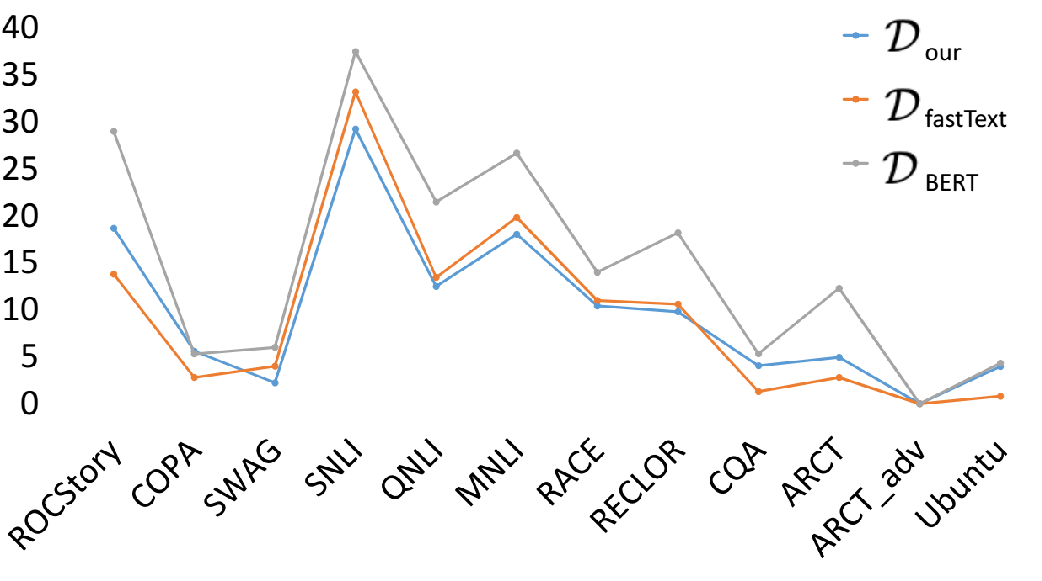
\includegraphics[width=0.7\columnwidth]{picture/d_figure.pdf}
%\caption{Deviation scores for three prediction models on all 12 datasets. 
%``Our'' means our logistic regression model.}
%\label{fig:d_figure}
%\end{figure}

%of $w$ with respect to label $l$ as
%%\KZ{Consider changing $\mathcal{F}$ to $\mathcal{B}$ to avoid confusion with $f$?}
%
%\begin{equation}
%    f_{\mathcal{F}}^{l} = f_{\mathcal{F}}(w, l),    
%\end{equation}
%%We call $f_{\mathcal{F}}^{(k,l)}$ \textit{cue metric}, 
%where $f_{\mathcal{F}}^{l}$ is a function which measures how much spurious information can be conveyed by token $w_k$ for a particular label $l$. 
%$\mathcal{F}$ is a set of cue metrics that we used for computing the \textit{cue score}. 

\subsubsection{Sentiment}

We assign sentiment features as 
positive, negative, or neutral to each hypothesis $h$: 
$sentiment(h) = \sgn(\mbox{num of positive words} - \mbox{num of negative words})$.
%in the hypothesis.
The sentiment polarity of a word
is determined by a look-up from pre-trained
sentiment lexica\footnote{NLTK: \url{https://www.nltk.org}}. 

\subsubsection{Tense}

Considering that the temporal order of events can be also 
important information for inference tasks, we include 
\textit{past}, \textit{present}, \textit{future} as Tense features. 
The tense is determined by verb tags after POS tagging.

\subsubsection{Negation}

Much work has observed that strongly negative words (``no'', ``not'') 
cause the model to predict contradiction for
neutral or entailed statements. Thus we think negation feature can be a factor which affects models in decision-making. 
Negation is decided by dependency parsing~\footnote{Scipy: \url{https://www.scipy.org}}.

\subsubsection{Overlap}
In many cases, substantial word-overlap between the premise and the
hypothesis sentences causes wrong entailment prediction, 
even if they are unrelated. 
%Very little word overlap causes a prediction
%of neutral instead of entailment. 
Thus we wonder 
whether overlap feature really influences models. 
We filter stop words, for example ``a'' and ``the'', before investigating overlap feature. 


\subsubsection{NER}
%\KZ{Rephrase this: The failure for the NER tests in CheckList
%indicates that these models are relying on shortcuts.}
Checklist constructs some stress tests for some NER features. The performance 
of models dropped heavily which indicates that these models are not robust and may 
take advantage of shortcuts.
For example, some name like ``Tom'' mostly appears with label ``contradiction'' 
may influence the decision of models.
%For example anchoring on named entities too strongly
%instead of understanding the reasoning behavior. 
We take NER features, like \textit{location}, \textit{person}, \textit{orgnization}, in our feature test.

\subsubsection{Typos}
The premise or the hypothesis is ill-formed because of spelling errors. 
Typo feature may also be learned by models as off-site information. 
We use a pretrained spelling model~\footnote{\url{https://github.com/barrust/pyspellchecker}} 
to detect the typos in a sentence. 

%We only pay attention to the features which have enough test data for model evaluation.
%In addition, we can analysis the credibility of test data through 
%the Kullback-Leibler (KL) Divergence. If a train dataset distribution is unbalance, 
%a similar distribution between train and T
%test can lead to insufficient test which test the cues mostly with a certain label. 

%\subsection{Data Set Filter}
%\label{sec:generate}
%Given the features $F$, 

%distribution and red distribution represent  the training and test data 
%distribution on the predication values respectively.  
%We use mean square error (MSE) to measure the balance 
%of a feature in a dataset. If the filtered training data distribution is 
%unbalanced on a feature, this feature can be seen as bias.  
%If this bias also exists in test data, indicating 
%a similar distribution exists in the test data, 
%this feature is considered a cue. 

%We show the distribution of some filtered SNLI datasets 
%in~\figref{fig:dataset_result}. 
%We can see that Word feature ``speaking'' mostly correlates with 
%label ``entailment''. So ``speaking'' is a bias. 
%The similar shape between the training and test data distribution indicates 
%this bias is a cue. Low Jensen-Shannon Divergence (JSD) score between the two
%distributions re-affirms our conclusion. 
%Compared with ``speaking'', Word feature ``pushing'' has lower MSE 
%score, but is still much higher than average distribution.  
%Thus ``pushing'' is also a bias. However we can observe that there is little similarity between 
%the train and test distribution. Therefore ``pushing'' is not a cue.
%With filtering and visualizing, we can analysis the biases 
%and cues in datasets. 
%Biases can influence models and cues make the evaluation unauthentic. 

%\begin{figure}[th]
%\centering
%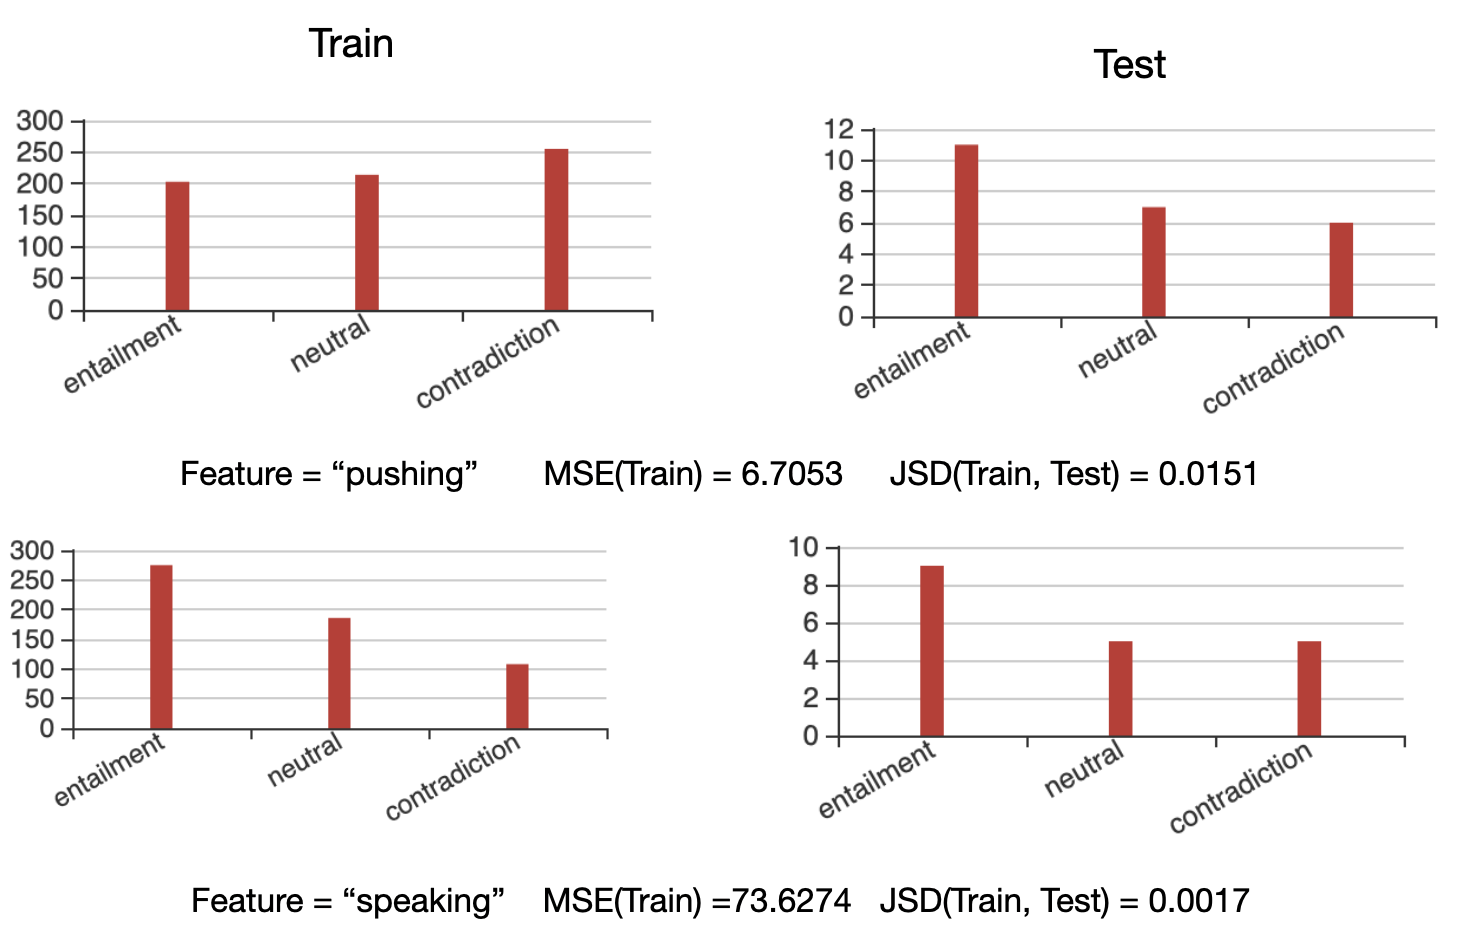
\includegraphics[width=1.0\columnwidth]{picture/dataset_result.jpg}
%\caption{Two examples of dataset distribution on features.}
%\label{fig:dataset_result}
%\end{figure}

\subsection{Model Evaluation}
\label{sec:model}

%We filter cases with specific features $F$ from the training and test data. 
For a specific feature, we filter the examples related to this feature from training and test dataset in~\figref{fig:framework}. 
For example, if we concern about ``Negation'' feature, we will extract all samples which contain negation tags on its parse tree. We can get feature distribution of filtered training data based on each label which is used as a reference for the model prediction distribution. The filtered test data is used to generate stress test that will be introduced in the following. 
In this filtering process, we don't retrain the model or change 
the parameters of models.

%Similar to discovering biases and cues, 
For investigating the bias of models, we can probe models by  
comparing the distribution of the model prediction results and 
the training data. We use JSD here to represent the deviation. 
The smaller the value of JSD, the more the model is affected 
by the distribution of training data.
%but don't provide new method for data augmentation. 
%We require a more fair dataset to test if a model is sensitive to a feature. 
The filtered test dataset of a feature in \figref{fig:framework} (red) is unbalanced among 
labels. The number of cases for each label can be denoted as $c_{ent}, c_{neu}, c_{con}$~(in 
SNLI task). If any of these number is smaller than a threshold $\sigma$, 
we won't consider this feature as a cue at all, because
 this feature is not well supported by enough data. 
%If the smallest number of samples among different labels is lower than 
%a threshold $\sigma$, we won't consider to test this feature. Because
% this feature is not well supported by enough data. 
%The smallest number can be denoted as $c_{min}=min(c_{ent}, c_{neu}, c_{con})$.
The maximum number can be denoted as $c_{max}=max(c_{ent}, c_{neu}, c_{con})$.
To make the result more intuitive and fair, 
we flatten the distribution by repeating $c_{max} - c_{l}$ cases from the filtered cases with label $l$ 
resulting in the orange ``stress test'' 
in \figref{fig:framework}. 
Then we test the model on this stress test. 
The similarity between prediction result (green) and 
training data distribution (blue) on a feature indicates how the model 
is influenced by the appearance of this feature in training data. 
For example, in \figref{fig:model_result}, we use 
ESIM~\cite{chen2016enhanced} model on SNLI. 
We can find that the model is affected by some bias features. 
Given ``pushing'', it still prefers to choose \textit{contradiction}. 
Further, it prefers to choose \textit{entailment} or \textit{neutral} with ``speaking''.  
JSD score for these two examples are also very low. 
%With comparison, we can find that models are sensitive to some bias features. 

%It is insufficient for testing if the filtered test data size is quite small or samples on 
%some label is rare which bellow a threshold $\sigma$. 
%Thought we can't generate cases for feature, we can point out what kind of 
%test samples should be augmented. 

\begin{figure}[th]
\centering
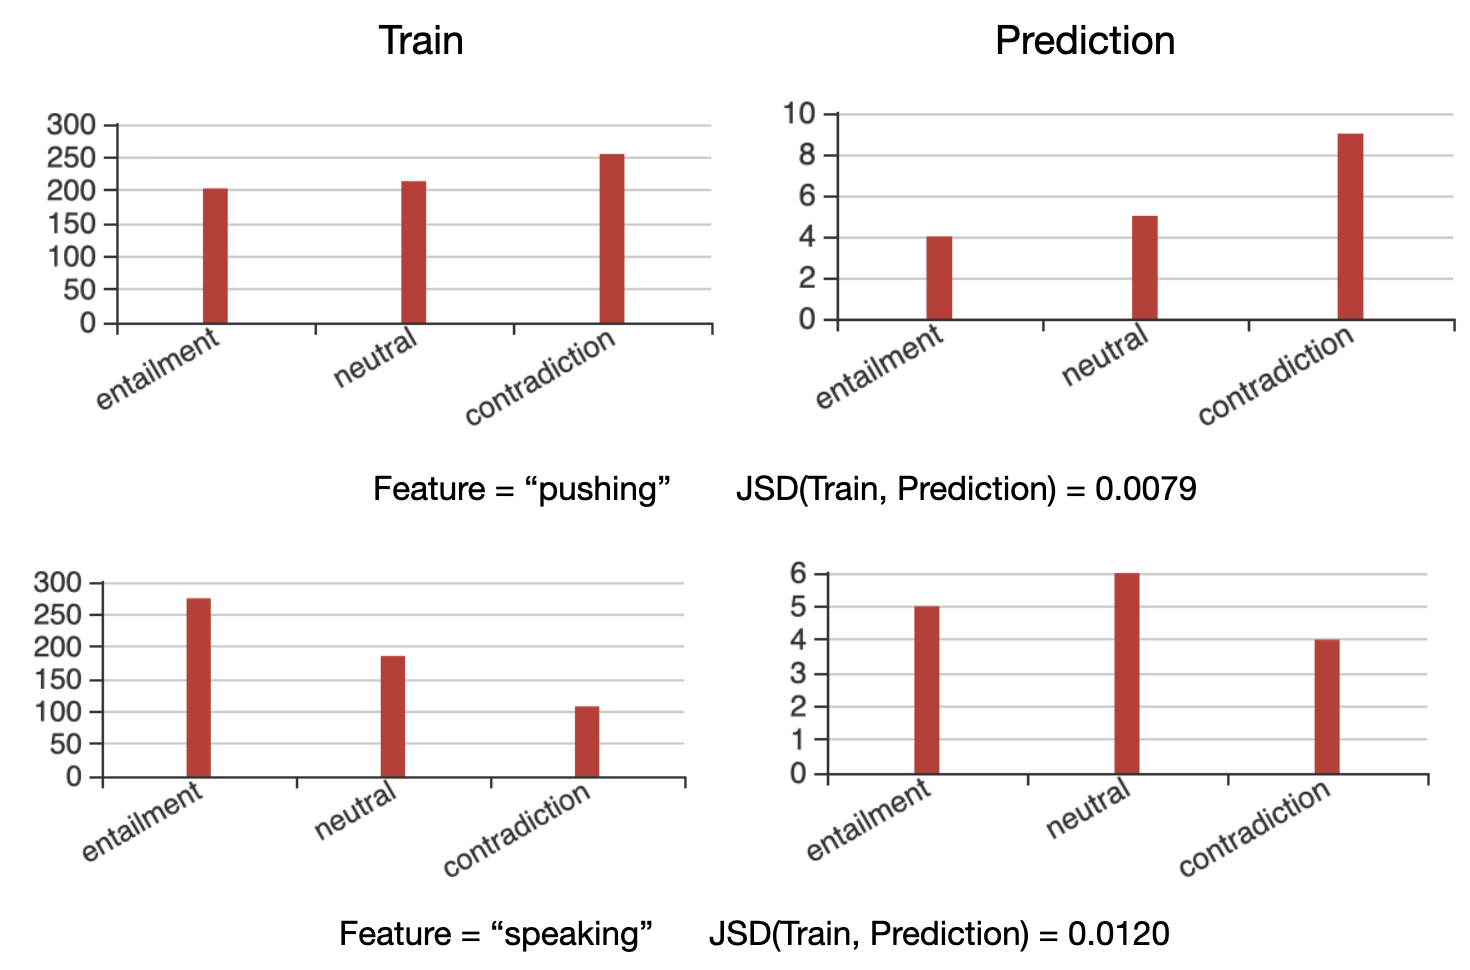
\includegraphics[width=1.0\columnwidth]{picture/model_result.jpg}
\caption{Two examples of model prediction result distribution on features.}
\label{fig:model_result}
\end{figure}


%The similarity is 
%calculated by Kullback-Leibler (KL) Divergence.


\section{Head Mapper}
%	* high order feature: arc heat change, influence of 2 order feature, feature template
%	* learning: MIRA, converge of training
%	* pseudocode of mapper(avoid circle) framework
%\KZ{Rephrase the following. What do you mean by attach? Also try not to be too casual, e.g., think about...}
%\BF{Mcdonald's example graph of decoding: ROOT John saw a dog yesterday which was a Yorkshire Terrier.}
In this section, we first give an example to explain how head mapper actually works. Then we explain
the features and scorer embeded in the head mapper. Finally, we describe the method to train the scorer model.

%\KZ{Figure needs to be restored to original one as some letters are missing.}

\begin{figure*}[th]
\centering
\epsfig{file=exampleparse_chg.eps, width=1.8\columnwidth}
\caption{Example Parse of head mapper}
%for the sentence ``\emph{John saw a dog yesterday which was a Yorkshire Terrier}". Red node is the child to be processed in every step; red arc is the final attachment from head to its dependent and dashed arc is left out to avoid circle in the parse tree.}
\label{fig:egparse}
\end{figure*}

\subsection{Parsing}
\figref{fig:egparse} shows the decoding process of the head mapper
for a non-projective example sentence previously used \cite{mcdonald2005non}.
%\KZ{You don't have to repeat the CoNNL format. It's not important.}
%Pseudocode shows how the head mapper works.
%Our decoder works just as the process in \figref{fig:egparse}.
%\BF{pseudocode of head mapper decoding and symbol explainations here}
A head mapper takes lexical information of a sentence and
a permutation sequence of words in that sentence as inputs.
The sequence of the sentence is:% from MaltParser:
$John_{1}\rightarrow a_{3}\rightarrow dog_{4}\rightarrow yesterday_{5}\rightarrow Yorkshire_{9}\rightarrow a_{8}\rightarrow was_{7}\rightarrow which_{6}\rightarrow Terrier_{10}\rightarrow saw_{2}$.
In step one, we look for the head of \textit{John} and
all the other words are potential candidate head. In order to measure
the probabilities of these candidate arcs, we introduce a scorer which
is the key idea of graph-based parsers. Judging from the scores
printed on every black arc in \figref{fig:egparse},
the red arc was eventually selected, i.e. $saw$ is taken to be the head
of $John$.  The process continues for the word \textit{a}, etc.

In practice, we maintain a disjoint set to ensure that
there are no cycles generated while parsing (e.g., in step 3 of
\figref{fig:egparse}),
so that the output is a dependency tree structure starting from
the ROOT node\footnote{A manually introduced node in dependency parsing task,
it is the root of a dependency tree}.
We also build a parse agenda to record the existing arcs which
provides the high order information for our scorer.
For a sentence with $N$ words, the final result consists of
($N+1$) nodes and constructed $N$ arcs.
%\KZ{You don't need to remind people over and over again this is a combination of
%MST and Malt. You just say what you did, if it's something that MST and Malt have
%done before, be very brief about this part, and give a citation. This paper
%is about your work, not about MST or Malt.}
%Both MaltParser and MSTParser treat projective and non-projective dependency tree discriminatively. MaltParser define an extra action SWAP to generate projectivization transformation of a non-projective dependency tree \cite{nivre2009non}.
%There is a drawback of MaltParser that it cannot generate non-projective output providing projective training set, because there are no SWAP action in oracle transitions. It is sensible to look into the relation between
%possible word pairs directly. But word order limits the word pairs considered in MaltParser. MSTParser employ Chu-Liu-Edmonds algorithm to decode non-projective cases \cite{mcdonald2005non}
%and Eisner algorithm to deal with projective trees\cite{mcdonald2005online}. Though Chu-Liu-Edmonds algorithm is a solution to unify projective and non-projective cases, it declines the accuracy while applying on projective trees. Our decoder also unifies these two situations and
%searches heads globally. It directly measures the relative closeness between every possible head and current processing word and generate non-projective tree naturally.
%Head mapper tries to map head for every word stepwise according to a given process sequence of words.
%\KZ{It makes sense to include an example here to illustrate the head-mapper.}

\subsection{Scorer and features}
%In order to simulate this process,
We introduce a linear arc scorer to measure the score of a directed arc.
The sum of all arc scores gives the final score of the whole parse tree.
%\BF{formula of arc score model}
%\[
%\text{Score}(\mathbf{y})=\displaystyle{\sum_{(i,j)\in\mathbf{y}}} \mathbf{w} \cdot \mathbf{f}(i,j)
%\]
%In this formula, $i,j$ are the indexes of an arc in parse tree $\mathbf{y}$. The inner product of arc feature vector $\mathbf{f}(i,j)$ and weight vector $\mathbf{w}$ represents score of an arc $(i,j)$. By summing up all the
%arc scores, we can get final score of the whole parse tree $\mathbf{y}$.
We currently use the same set of high-dimensional binary features as MSTParser,
%\BF{feature template table}
including second order features \cite{mcdonald2006online}.
%As the previous statement, feature scope in graph-based parser
%is limited by decoding algorithm and several works successfully
%adapt Eisner algorithm to include high order features .
Because of the deterministic decoding in our framework,
we can make use of existing arcs to guide later head mapping.
This kind of decoder gives us the flexibility of applying any
high order features explored by previous
works~\cite{carreras2007experiments,koo2010efficient,ma2012fourth}.

\subsection{Learning algorithm}
%\KZ{Again, you are making it sound like you only did some minor changes to MST.
%This is not the right style to write about your work. You can say we use a modified
%verion of MIRA~\cite{}, in which we did blah..}
%Based on different decoding and factoring methods, graph-based models employ different learning algorithms to induce the feature weights. Among them, variant perceptron algorithms are widely used \cite{kubler2009dependency}.
In this work, we adopt the iterative online training framework MIRA
(Margin Infused Relaxed Algorithm), which was used in the training process
of MSTParser. The updating constraint is defined as
\begin{align*}
&\text{min}\|\mathbf{w}^{(i+1)}-\mathbf{w}^{(i)}\|\\
&\text{s.t. } s(\boldsymbol{x}_t,\boldsymbol{y}_t)-s(\boldsymbol{x}_t,\boldsymbol{y}')\ge L(\boldsymbol{y}_t,\boldsymbol{y}')
%\\&\forall \boldsymbol{y}'\in \text{dt}(\boldsymbol{x}_t)
\end{align*}
where $\mathbf{w}^{(i)}$ are the feature weights for the $i$-th iteration,
$\mathbf{x}_t$ and $\mathbf{y}_t$ are sentence and its gold parse tree,
respectively. $\mathbf{y}'$ is the output of our parser with $\mathbf{w}^{(i)}$ and
score margin is given out by a loss function $L$.

%On each update, MIRA attempts to keep the norm of the change to the parameter vector as small as possible, subject to
%correctly classifying the instance under consideration with a margin at least as large as the loss of the incorrect classifications \cite{mcdonald2005online}.
%\BF{this is the original sentence in this paper}
%Similarly, we define the loss function as the number of incorrect arcs to apply MIRA to dependency parsing and it
%is represented as following formula: \BF{Is this formula necessary ?}
%\BF{MIRA formula}
%\KZ{Don't like the following sentence.}
%From this definition, the only change we should make is replacing the exact inference decoder with our deterministic
%decoder.
Every time, we update the feature weights based on one sentence. The
decoder gives a greedy parse according to current feature weights.
By scoring the gold dependency tree and the current parse,
along with the number of incorrect arcs in the current parse,
MIRA updates to eventually converge to an optimal scorer.
The learning algorithm typically terminates after a few iterations.
%(\figref{fig:itertest}).
%\BF{Converge graph of head mapper}
%\begin{figure}[htp]
%\centering
%\epsfig{file=itertest.eps, width=\columnwidth}
%\caption{Accuracy curves on training set. \newline Test on first 100 sentence of WSJ senction 00.}
%\label{fig:itertest}
%\end{figure}


\section{Sequence Predictor}
%A sequence predictor either selects the word to process stepwise, or generates an complete word sequence.
We developed two types of sequence predictor. The first type is based on
offline training from ``gold'' parsing sequences, and produces a complete
parsing sequence given a sentence. The second type is unsupervised and is
integrated with the decoding process, i.e. it produces the next word to
process based on the current parsing configuration.
We divide the first type of predictor into two approaches, one by a learning
to rank algorithm, and second by an action classifier used in MaltParser.
Next we briefly discuss these three approaches.

%We state the rule of gold sequence in Section 2 and we can generate gold sequences with the gold dependency trees.
%Sequence predictor then learns from these gold sequences and tries to produce a sequence
%for new sentences.
%
%\subsection{Effects of Sequences}
%\KZ{Not sure what ``Sequence dependence'' means. Headings should be self-explanatory
%and clean. Consider rephrase the following paragraph. Very garbbled.}
%As we point out in section 2, getting a gold sequence from a gold dependency tree is not a one-to-one mapping.
%\BF{breadth-first traversal and malt convert sequences of example sentence}
%For example, there is a breadth-first traversal sequence of the sentence in \figref{fig:egparse},
%$which_{6}\rightarrow was_{7}\rightarrow a_{8}\rightarrow Yorkshire_{9}\rightarrow a_{3}\rightarrow Terrier_{10}\rightarrow John_{1}\rightarrow dog_{4}\rightarrow yesterday_{5}\rightarrow saw_{2}$
%, which is also a gold sequence along with the example sequence.

\subsection{Pairwise learning to rank}
\cut{In this approach, we attempted two ways to generate gold parsing sequences.
First is a bottom-up, breadth-first traversal of the gold parse tree. This
way we are essentially processing words which are lower down in the parse
tree first, which are often less important modifiers, before moving to words
which are more central to the syntactic structure of the sentence.
The second is to take the training data from a converting function of
MaltParser, which converts a gold parse tree into a sequence of actions.
We can infer the parsing sequence of words from the sequence of actions.}

%We human beings execute a few pairwise comparisons to decide the next
%word to be processed, which is similar to preference learning problem in learning to rank.
%Sequence predicting is also a ranking process. We select next word to process by comparing it with the other words in a pairwise way.
%Viewing the task of sequence predictor in this way,
%preference learning problem in learning to rank gives a solution to predict.
We can decompose a gold sequence into pairwise partial orders between
two words and train a binary classifer to determine the order of any two
words within a sentence. This is a popular approach in learning to rank.
However, combining pairwise orders into a complete sequence is an NP
problem~\cite{grotschel1984cutting}, we therefore use a greedy algorithm
from Cohen \cite{schapire1998learning} to produce such a sequence.

\subsection{Action classifier in MaltParser}
MaltParser employs a classifier to determine what parsing action (e.g.,
{\em shift}, {\em push}, etc.) to take at each step. The whole parsing
process defines a sequence of such actions. Although this sequence is
not exactly the word sequence used in our system, such a word sequence
can be inferred rather straightforwardly from the action sequence.
Another advantage of
the MaltParser is that it's extremely fast. Therefore, we can use MaltParser
to quickly parse through a given sentence, record the action sequence and
infer the parse sequence from it.

%
%Inspired by our left-to-right analysis of a sentence, we either find
%head for current word or skip this hard word and scan on. This is obviously a classification problem and
%MaltParser happen to hold the same view.\BF{cannot say so now} MaltParser add arc incrementally and provide us a potential sequence.
%In fact, we can understand the action classifier in a different way that it can reflect the relative
%priority between the top two words on processing stack. So, we translate the action as:
% LA - process the word on the top of stack;
% RA - process the second word in stack;
% SH - postpone the process of both the two words on top of stack.


%We can decompose the predicting process into two steps:
%getting pairwise rank of every two nodes and aggregating
%these partial results into a complete process sequence.
%
%We apply LIBLINEAR\footnote{\urlstyle{same}\url{http://www.csie.ntu.edu.tw/~cjlin/liblinear/}} to training a binary classifier to get the priority of every two words. The training data are pairwise orders extracted from the gold sequence.
%The classifier can then be used to predict the relative ordering for any two words with a confidence score.
%\BF{Jia fill the details: rankSVM, Cohen, citation of preference learning}

%  \item {\bf Malt} The oracle sequence generated by converting function in MaltParser.
%  \item {\bf Random} A random permutation sequence of words for a sentence.
%  \item {\bf Increase} The left-to-right sequence, which means we process the sentence with
%  the word index increasing.
%\end{itemize}
%
%In order to test how the sequence quality influence decoding and measure different types of sequences,
%we generate four types of sequence files to test on the head mapper.
%%The train set is transformed by StanfordParser on WSJ section 2-21 and test set on WSJ section 00-01.
%Types of sequences are list below:
%Among them, the Malt sequence outperforms other types of the sequences.
%In the following, we describe a few alternative approaches to predict the sequences.
%%        \item[1] The breadth-first traversal sequence of a sentence
%        \item[2] The oracle sequence generated by converting function in MaltParser.
%        \item[3] Predicting process sequence of MaltParser stackproj algorithm.
%        \item[4] The random permutation sequence of words in a sentence.
%        \item[5] The left to right sequence, word indexes are process sequences.
%{\bf Breadth-first} The breadth-first traversal sequence of a sentence.
%
%{\bf MaltConvert} The oracle sequence generated by converting function in MaltParser.
%
%{\bf MaltPredict} Predicting process sequence of MaltParser stackproj algorithm.
%
%{\bf Random} The random permutation sequence of words in a sentence.
%
%{\bf Increase} The left to right sequence, word indexes are process sequences.
%{\small
%~\\
%
%$\bullet$ Oracle {\bf converting} sequences of MaltParser.
%
%$\bullet$ {\bf Breadth-first} traversal of a gold parse tree.
%
%$\bullet$ {\bf Predicting} process sequence of MaltParser.
%
%$\bullet$ A {\bf random} words permutation of the sentence.
%
%$\bullet$ A word sequence with {\bf increasing} index from left to right of the sentence.
%\begin{table*}[htbp]
%  \centering
%  \caption{Cross test of sequence type}
%  %\begin{threeparttable}
%    \begin{tabular}{Il|cccccIccI}
%    \whline
%    %\diagbox{Test}{Train}& Breadth-first\tnote{1} & MaltConvert\tnote{2} & MaltPredict\tnote{3} & Random\tnote{4} & Increase\tnote{5} & Average & StdDev \\
%    \diagbox{Test}{Train}& MaltConvert & Breadth-first & MaltPredict & Random & Increase & Average & StdDev \\
%    \hline
%    MaltConvert & 93.59\% & 67.32\%  & 93.29\% & 89.50\% & 83.91\% & 85.52\% & 0.109 \\
%    Breadth-first & 79.65\% & 92.36\% & 80.93\% & 86.46\% & 84.75\% & 84.83\% & 0.050 \\
%    MaltPredict & 89.30\% & 66.07\%  & 89.50\% & 87.14\% & 82.36\% & 82.87\% & 0.098 \\
%    Random & 55.41\% & 48.84\% & 56.49\% & 70.92\% & 62.77\% & 58.89\% & 0.083 \\
%    Increase & 48.89\% & 46.98\% & 48.83\% & 65.18\% & 63.36\% & 54.65\% & 0.088 \\[2pt]
%    \whline
%    \hline
%    %\midrule[3pt]
%    %     &       &       &       &       &       &     &  \\
%    Average & 73.37\% & 64.31\% & 73.81\% & 79.84\% & 75.43\%      &     & \\
%    StdDev & 0.201 & 0.183 & 0.200 & 0.110 & 0.113     &     & \\
%    \Cline{1.5pt}{1-8}
%    \end{tabular}%
%    %\begin{tablenotes}
%%        \footnotesize
%%        \item[1] The breadth-first traversal sequence of a sentence
%%        \item[2] The oracle sequence generated by converting function in MaltParser.
%%        \item[3] Predicting process sequence of MaltParser stackproj algorithm.
%%        \item[4] The random permutation sequence of words in a sentence.
%%        \item[5] The left to right sequence, word indexes are process sequences.
%%      \end{tablenotes}
%%\end{threeparttable}
%  \label{tab:crosstest}%
%\end{table*}%
%\subsection{Attempts}


\subsection{Feature score based predictor}
%{\bf Scorer-based  }
The intuition of sequence predictor is to rank words
according to the ease of head word attaching.
Words that are easy to handle can be processed earlier without high order features.
\cut{Words that are processed later are harder and may require high order
features. Such high order features are available later because many arcs
have been attached by then.}
Since the head mapper can score every possible arc,
for each word $w$, we can compute a list of scores for all the candidate
head word of $w$. If there is a large difference in scores between the best
candidate head word and the remaining candidates for $w$,
then we can conclude the processing $w$ doesn't require high order features
and therefore can be done early.
%this score naturally reflects the possibility that
%a certain word can be the head of another word. We consider a word to be
%easy to deal with if
%A word is easy to deal with means that there is a head candidate much more possible than other candidates, so that it is no need to employ higher order features to find a head. In other words, greater the difference is, harder can higher order features make up for the difference.
%The intuition of sequence predictor is ranking words according to the ease
%of head word attaching. Now that the head mapper can score all possible
%head words and then choose the one with highest score, this score
%can be seen as the confidence of this arc. An arc with higher confidence
%is naturally easier to deal with.
%A word is easy to deal with means that there is a head candidate gets a higher score than the other candidates.
\cut{
As such, we maintain a matrix $M_{(n+1) \times n}$ to store the scores of
head-dependent pairs, which are initially calculated by the first order
features. When a new arc is added to the parse tree, we remove the
cells that may form a cycle with the existing arcs and update the cells
relating to this new arc using higher order features.}
%Each time we choose the word with greatest difference between its highest score and second highest score.
%After we build an arc,
 %and update sibling scores (different high order structures may require more updates).

We will compare these three approaches in some preliminary evaluations next.



%~\\
%}
%\BF{table of cross test}

%The result of this cross test is in \tabref{tab:crosstest}. As we can
%see, training result relies much on the sequence information. Breadth-first sequence
%and MaltConvert sequence are both gold sequence of a sentence. These gold sequence models
%cannot obtain the best accuracy in other types of test sequence. Instead, the accuracy is determined
%by two factors. One is the quality of sequence, the other is matching degree between train
%sequence type and test sequence type. We can also tell from this table that we can get a
%high accuracy with a good type of sequence even on our greedy head mapper.
%
%The average accuracy and standard variance for sequence type of train file indicates the
%ability to match other types of sequence. Better sequence type gets a higher
%standard variance and a lower average accuracy. Random sequence approaches to all types in
%some sub-sequences. Increase sequence approaches to the two gold sequence because their nodes
%in the same level on gold trees mainly follow a left-to-right process rule.
%
%However, the average accuracy and standard variance for sequence type of test file shows
%the quality of a sequence type. Worse types of sequence struggles in parameter updates
%in training and better types test file can obtain a not bad result on models of worse types.
%On the contrary, worse types get bad performance on models of better types. So the accuracy
%of test file is limited by the quality of sequence type.
%%\BF{interesting conclusions: in Report201516doc, good order+ greedy head mapper->good result}
%
%Further, we print out the first-order arc heat map of same sentence.
%\BF{arc heat map}
%As we can see, different models score the arcs quite differently. Scorer relies much on the sequence and
%matched sequence pattern in train set and test set promise a high accuracy, which makes sequence predictor
%an interesting but hard task.


\section{Experimental Results}
\label{sec:eval}
In this section, we first present the data set, 
then compare the fuzzy match results
of the ODL system with three other competing methods, before evaluating the
effects of incremental manual correction strategies.

\subsection{Dataset and Preprocessing}
%\JY{
%The dataset that we used for evaluation comes from real life ECG reports. 
%These reports come from different hospitals recorded at different times
%and they can be divided into many different formats. 
%For our experiment, we choose four different formats. 
%The examples about these formats are shown in \figref{fig:dataset}.
%One of the reason that we choose images in these four formats is 
%these four formats have the largest number of images. 
%Another reason is they contain different attributes, languages, and so on.
%}
The dataset we use are from real ECG reports, and are recorded at 
different times and different hospitals. Those reports can be 
divided into several different categories. We chose four typical kinds 
of reports which include many images and contain much useful information 
such as attributes, languages so that we could extract more data 
from them (see \figref{fig:dataset}).
% and they can be divided into four different formats with examples shown in \figref{fig:dataset}. 
The statistics about our dataset is shown in \tabref{tab:statis}. 

\begin{figure}[th]
\centering
\subfloat[Format 1]{
\label{fig:dataset:1}
\epsfig{file=figure/f1.eps, width=0.24\columnwidth}
}
% \hfill
\subfloat[Format 2]{
\label{fig:dataset:2}
\epsfig{file=figure/f2.eps, width=0.24\columnwidth}
}
%\hfill
\subfloat[Format 3]{
\label{fig:dataset:3}
\epsfig{file=figure/f3.eps, width=0.24\columnwidth}
}
\subfloat[Format 4]{
\label{fig:dataset:4}
\epsfig{file=figure/f4.eps, width=0.24\columnwidth}
}
\caption{Examples of Four Kinds of ECGs}
\label{fig:dataset}
\end{figure}

\begin{table}[th]
\centering
\caption{Statistics for The Dataset}
\label{tab:statis}
\begin{tabular}{|c|c|c|c|c|}
\hline
Format & 1 & 2 & 3 & 4\\
\hline \hline
Number of Images & 124 & 113 & 102 & 97\\ 
\hline
Number of Attributes per Image & 17 & 16 & 18 & 15 \\
\hline
\end{tabular}
\end{table}

As the examples shown, these ECG images are in different colors 
and have many noises like grid lines. 
Because these variations and noises affect the performance of the OCR engine, 
we preprocess the images into a clean version. 
The detailed techniques are discussed in \secref{sec:discuss}. 

% we use auto thresholding to 
% preprocess the images to remove the noisy lines and 
% turn the color images into black and white. 
% An example of the preprocessing result is shown in \figref{fig:preprocess}. 
% Auto thresholding is to segment the images based on the colour 
% features automatically. In our system we make use of the tool 
% ImageJ\cite{schneider2012671} to do the preprocessing.  
% \begin{figure}[ht]
% \centering
% \subfloat[Before Preprocessing]{
% \label{fig:preprocess:1}
% \epsfig{file=figure/f1.eps, width=0.48\columnwidth}
% }
% % \hfill
% \subfloat[After Preprocessing]{
% \label{fig:preprocess:2}
% \epsfig{file=figure/pref1.eps, width=0.48\columnwidth}
% }
% \caption{Results of Preprocessing}
% \label{fig:preprocess}
% \end{figure}

\subsection{Extraction Accuracy}
Next, we compare our method with three competing methods.
The first and most naive method for information extraction from medical images 
is to write a simple parser for the XML results of the OCR engine. 
We consider this approach to be the baseline for 
evaluation. In this parser, we didn't include any fuzzy matching 
strategies, but instead extracted all results using exact matches. 

The second competing method involves marking all zones of interest 
on images and getting all the OCR results in them. 
To adjust the small changes of 
zone areas between images, a marker zone is set so that 
all other zones of interest can be adjusted against it as
a reference point. 
An example image after being marked with the zones of interest 
and the marker zone is shown in \figref{fig:zOCR} (Zones of interest 
are in blue and the marker zone is in red).

\begin{figure}[th]
\begin{minipage}{0.5\columnwidth}
\centering
\epsfig{file=figure/17_zOCR.eps, width=0.7\columnwidth}
\caption{Image Marked With Zones}
\label{fig:zOCR}
\end{minipage}
\begin{minipage}{0.5\columnwidth}
\centering
\epsfig{file=figure/17_pl.eps, width=0.7\columnwidth}
\caption{Page Layout Analysis Result}
\label{fig:pl}
\end{minipage}
\end{figure}

The third approach is to use the page layout analysis 
technique \cite{o1993document}. 
This method is used to determine where the text 
resides on a page. 
By this method, the hierarchy of physical components 
can be generated against which we can match the predefined 
hierarchy of logical components. An example result of our page layout 
analysis is shown in \figref{fig:pl}.

\begin{figure}[th]
\centering
\epsfig{file=figure/2_pl.eps, width=0.5\columnwidth}
\caption{An Error Page Layout Analysis Result}
\label{fig:errorpl}
\end{figure}


The results of comparison are shown in \tabref{tab:compare}. 
We only calculated the accuracies for extracting the results of 
variables since we already know the exact values of constant 
expressions. Based on our experiment, our method of fuzzy matching 
outperforms all other methods on all 4 types of ECGs. 
The reason is that zonal OCR and page layout analysis are highly 
related to image processing in order to extract data. The accuracy of 
zonal OCR is greatly affected by the setting of zones of interest. 
If the zones of interest are too large, it's possible that noises are
also extracted; while if the zones of interest are too small, results 
can be incomplete. For page layout analysis, the accuracy is 
affected by the granularity of the page layout unit and the 
misrecognition affects the matching with the predefined 
hierarchy of logical components. For our method, the smallest 
unit is word in text so our description can be very accurate. 
At the same time, the fuzzy matching strategies also enable 
the description to omit some unnecessary details.
% \KZ{Need focus on explaining why we are only slightly better, and what are
% the problems of the other three methods, despite that their accuracies are
% not that bad! e.g., efforts to mark the zones, I'm still not convinced
% how come without fuzzy match, zonal methods can be so good since the dist
% between the marker zone and the interesting zones can be slightly off in each
% image.}   

Even though the two competing approaches seem just marginally outperformed
by our fuzzy matching approach, these two approaches have their own 
important limitations. 
In a zonal OCR, it's important to adjust the zones of interest 
based on the marker zone. Misrecognition of the marker 
is disasterous, as all the extracted information will be incorrect. 
The other approach, page layout analysis, requires analyzing 
the text boxes in images before conducting logical labeling. 
If the text boxes are recognized incorrectly, some of the
important information may be omitted from output. 
As shown in \figref{fig:errorpl}, 
text box recognition errors cause the OCR to overlook the unit and 
other valuable information. 
However, the fuzzy match design of our system can 
tolerate these types of errors that the OCR engine often makes. 
We seek to find an optimized solution which can extract 
correct information as much as possible. 


\begin{table}[th]
\centering
\caption{Accuracy For Different Methods}
\label{tab:compare}
\begin{tabular}{|c|c|c|c|c|}
\hline
Format & 1 & 2 & 3 & 4\\
\hline \hline
Exact Match & 58.8\% & 56.3\% & 61.1\% & 53.4\% \\
\hline
Zonal OCR & 81.2\% & 79.8\% & 81.7\% & 80.6\% \\
\hline
Page Layout & 79.7\% & 80.2\% & 81.2\% & 81.1\% \\
\hline
Our Fuzzy Match & {\bf 85.5\%} & {\bf 83.8\%} & {\bf 84.9\%} & {\bf 84.0\%}\\ 
\hline
\end{tabular}
\end{table}

\subsection{Incremental Manual Correction}
%In this section, we compare the performance of 
%the human correction part in our system. 
%Another important part of our system is the human correction 
%process. By making use of the human power, we can correct 
%the errors that occur due to the OCR engine. 
We compare the two policies for recommending errors for manual correction, 
namely, random recommendation and most frequent error 
description element recommendation. The relationship between the 
amount of corrections and the accuracy of different types of 
ECGs are shown in \figref{fig:humancorr}. 
%For random correction, we randomly suggest that some errors be 
%corrected each time. 
%The accuracy of random correction is calculated by averaging 
%the results 100 times. For the most frequent error 
%description element recommendation, 
%corrections for most frequently made errors will be suggested first. 

%\KZ{Some of the words are incorrectly displayed in the following figures.}

\begin{figure}[!ht]
\centering
\subfloat{
%% \label{fig:hc:1}
\epsfig{file=figure/hcf1.eps, width=0.48\columnwidth}
}
% \hfill
% \centering
\subfloat{
% \label{fig:hc:2}
\epsfig{file=figure/hcf2.eps, width=0.48\columnwidth}
}
\hfill
% % \centering
\subfloat{
% \label{fig:hc:3}
\epsfig{file=figure/hcf3.eps, width=0.48\columnwidth}
}
% % \centering
\subfloat{
% \label{fig:hc:4}
\epsfig{file=figure/hcf4.eps, width=0.48\columnwidth}
}
\caption{Comparison of Two Correction Strategies in 4 Types of Images}
\label{fig:humancorr}
\end{figure}

% \KZ{Need to modify the figs so that lines don't touch into
% the legends, ad the caption don't overlap with the figs.}

As shown in \figref{fig:humancorr}, the more corrections we make, 
the better accuracy we get. 
The improvement to the accuracy rate is better 
when using the most frequent recommendation, compared with random 
recommendation. Using the most 
frequent recommendation is more effective, 
since we can correct more errors than random recommendation. 
With more corrections made, the improvement of 
accuracy tends to saturate, especially with regard to the 
most frequent error strategy. This is the effect of diminishing
returns, as corrections learned later tend to be minor ones and make
less impact to the overall performance.
% \KZ{Need to explain why there's only limited improvement after 15 corrections.
% Maybe because the data size is not big enough, so there's not many repeated
% errors?}
The improvement of accuracy is limited after 15 corrections. 
The main reason is that there are not many repeated errors due to 
the small size of the data set and furthermore, our system 
can only make corrections according to the correction model, 
which is sensitive to repeated errors.

% \begin{enumerate}
% \item Compare the description code with generated code to show our language is a simple one;
% \item Compare the accuracy with baseline, exact match on the OCR results, to show our language can tolerate the noises and errors;
% \item Compare the performance on different image formats;

% \item Compare the accuracy between our approach and others, including using related image position;


% \item Experiments about the relationship of the accuracy rate 
% and the number of errors corrected;

% \begin{table}[!hbp]
% \centering
% \caption{Most Frequent}
% \begin{tabular}{|c|c|c|c|c|}
% \hline
% Type & 1 & 2 & 3 & 4\\
% \hline
% Accuracy(0 errors) & 85.5\% & 83.8\% & 84.9\% & 84.0\%\\ 
% \hline
% Accuracy(1 errors) & 85.7\% & 84.0\% & 85.0\% & 84.2\%\\ 
% \hline
% Accuracy(5 errors) & 86.2\% & 84.6\% & 85.6\% & 84.8\% \\
% \hline
% Accuracy(10 errors) & 86.6\% & 85.2\% & 86.2\% & 85.5\% \\
% \hline
% Accuracy(15 errors) & 86.8\% & 85.7\% & 86.6\% & 85.9\% \\
% \hline
% % \caption{Most Frequent}
% \end{tabular}
% \end{table}

% 0 85.5 85.5
% 1 85.7 85.5
% 5 86.2 85.7
% 10 86.6 86.0
% 15 86.8 86.2

% 0 83.8 83.8
% 1 84.0 83.9
% 5 84.6 84.1
% 10 85.2 84.4
% 15 85.7 84.7

% 0 84.9 84.9
% 1 85.0 84.9
% 5 85.6 85.1
% 10 86.2 85.4
% 15 86.6 85.7

% 0 84.0 84.0
% 1 84.2 84.1
% 5 84.8 84.4
% 10 85.5 84.7
% 15 85.9 85.1

% \begin{table}[!hbp]
% \centering
% \caption{Random}
% \begin{tabular}{|c|c|c|c|c|}
% \hline
% Type & 1 & 2 & 3 & 4\\
% \hline
% Accuracy(0 errors) & 85.5\% & 83.8\% & 84.9\% & 84.0\%\\ 
% \hline
% Accuracy(1 errors) & 85.5\% & 83.9\% & 84.9\% & 84.1\%\\ 
% \hline
% Accuracy(5 errors) & 85.7\% & 84.1\% & 85.1\% & 84.4\% \\
% \hline
% Accuracy(10 errors) & 86.0\% & 84.4\% & 85.4\% & 84.7\% \\
% \hline
% Accuracy(15 errors) & 86.2\% & 84.7\% & 85.7\% & 85.1\% \\
% \hline
% % \caption{Random}
% \end{tabular}
% \end{table}


% \begin{figure}
% \centering
% \subfloat[ECG1]{
% \label{fig:hcre:a}
% \epsfig{file=figure/f1.eps, width=0.48\columnwidth}
% }
% \hfill
% \subfloat[ECG2]{
% \label{fig:hcre:b}
% \epsfig{file=figure/f2.eps, width=0.48\columnwidth}
% }
% \hfill
% \subfloat[ECG3]{
% \label{fig:hcre:c}
% \epsfig{file=figure/f3.eps, width=0.48\columnwidth}
% }
% \hfill
% \subfloat[ECG4]{
% \label{fig:hcre:d}
% \epsfig{file=figure/f4.eps, width=0.48\columnwidth}
% }
% % \caption{E}
% \label{fig:hcre}
% \end{figure}

% \item Compare different strategies for correcting errors, including most frequent error elements, most frequent error types.
% \end{enumerate}


\section{Related Work}
\paragraph{Clarification Question Generation} The concept of CQ can be naturally raised in a dialogue system where the speech recognition results tend to be erroneous so that we raise CQs for sanity check \citep{stoyanchev2014towards}, or the intents for a task is incomplete or ambiguous in a first short utterance and further CQs are needed to fill in the slots \citep{dhole2020resolving}. The concept is then extended to IR to clarify ambiguous queries \citep{aliannejadi2019asking}, and has been successfully put into practice \citep{zamani2020generating}. Other application areas including KBQA \citep{xu2019asking} and open-domain dialogue systems \citep{aliannejadi2020convai3}. CQGen can also be applied to help refine posts on websites like StackExchange \citep{Kumar_2020} and Amazon \citep{rao2019answer}. In this context, our work closely follows the research line of \citep{rao2018learning, rao2019answer, cao2019controlling}. \citet{rao2018learning} first adopted a retrieval-then-rank approach. They \citep{rao2019answer} then proposed a generation approach to train the model to maximize the utility of the hypothetical answer for the questions with GAN, to better promote specificity. \citet{cao2019controlling} propose to control the specificity by training on data with explicit indicator of specificity, but it requires additional specificity annotation. Towards the similar specificity goal, we adopted a different keyword-based approach. They also assume generating one question per context, which we claim is not sufficient to cover various possible information needs, and thus propose the task of the diverse CQGen.

\paragraph{Diverse Generation} The demand for diverse generation exists in many other fields~\cite{vijayakumar2018diverse, LiangZ18code, shen2019mixture}, and we've drawn inspirations from these literatures. For image captioning, we may use multiple descriptions for different focusing points of a scene. \textit{Diverse Beam Search} \citep{vijayakumar2018diverse} was proposed to broaden the searching space to catch such diversity by dividing groups in decoding and imposing repetition penalty between them. For machine translation, a context can be translated with different styles. \citet{shen2019mixture} thus proposed \textit{Mixture of Expert} models including hMup to reflect various styles with a discrete latent variable (\textit{expert}). And here for CQGen, diversity is required to cover various potentially missing aspects, so we come up with the idea to use keywords as a controlling variable like \textit{expert} to promote diversity.



\section{Conclusion}

In this paper, we incorporated the idea of Cookie Theft picture description task into the evaluation of the high-level cognitive abilities of LVLMs and designed a novel evaluation benchmark called CogBench.
% Images in CogBench are of high quality and require more cognitive reasonings to understand, which makes it different from existing image datasets.
The images in CogBench are of high quality and demand more complex cognitive reasoning for interpretation, setting it apart from existing image datasets.
% It consists of a image description task and a VQA task.
Experiments show that there is still a large gap between the cognitive abilities of LVLMs and human beings, indicating CogBench is a challenging benchmark.

% In the future

\bibliographystyle{acl}
\bibliography{parser}
\end{document}
